\documentclass[10pt,a4paper,oneside]{book}
\usepackage{listings}
\usepackage{multirow}
\usepackage[table]{xcolor}
\definecolor{tableShade}{HTML}{C5D5A9}
\definecolor{tableShade2}{HTML}{ECECEC}
\usepackage{shadow}
\usepackage[left=+2.2cm, right=+2.5cm]{geometry} 
\usepackage[T1]{fontenc}
\usepackage[pdftex]{graphicx}
\usepackage{relsize,fancyvrb}
\usepackage{fancyhdr}

% The package hyperref provides LaTeX the ability to create hyperlinks within
% the document
\usepackage{hyperref}
\hypersetup{
    colorlinks,%
    citecolor=black,%
    filecolor=black,%
    linkcolor=black,%
    urlcolor=black
}

\usepackage{eso-pic}
\newcommand\BackgroundPic{
\put(0,0){
\parbox[b][\paperheight]{\paperwidth}{%
\vfill
\centering
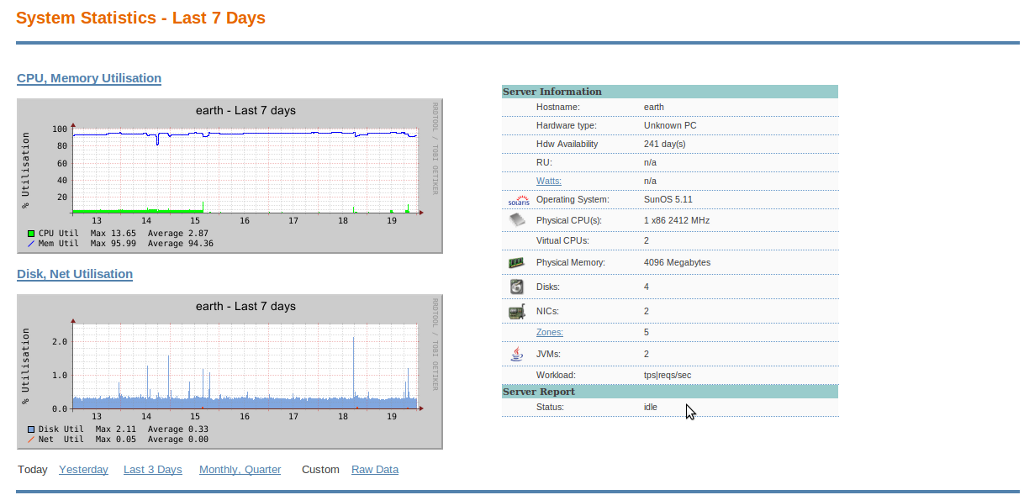
\includegraphics[width=\paperwidth,height=\paperheight,keepaspectratio]{back.png}
\vfill
}}}


\renewcommand{\rmdefault}{phv} % Arial
\renewcommand{\sfdefault}{phv} % Arial

\usepackage{color}
\definecolor{gray}{rgb}{0.4,0.4,0.4}
\definecolor{darkblue}{rgb}{0.0,0.0,0.6}
\definecolor{cyan}{rgb}{0.0,0.6,0.6}

\lstset{
  basicstyle=\ttfamily,
  columns=fullflexible,
  showstringspaces=false,
  commentstyle=\color{gray}\upshape
}

\lstdefinelanguage{XML}
{
  morestring=[b]",
  morestring=[s]{>}{<},
  morecomment=[s]{<?}{?>},
  stringstyle=\color{black},
  identifierstyle=\color{darkblue},
  keywordstyle=\color{cyan},
  morekeywords={xmlns,version,type}% list your attributes here
}


% %%%%%%%%% %
% FrontPage %
% %%%%%%%%% %
\makeatletter
\def\thickhrulefill{\leavevmode \leaders \hrule height 1pt\hfill \kern \z@}
\renewcommand{\maketitle}{\begin{titlepage}%
    \let\footnotesize\small
    \let\footnoterule\relax
    \parindent \z@
    \reset@font
    \null\vfil
    
\includegraphics[width=15mm,height=15mm]{sdrnew40x42.png}
    \begin{flushleft}
      \huge \bfseries \strut \@title \strut
    \end{flushleft}
    \par
    \hrule height 1pt
    \par
    \begin{flushleft}
      \bfseries \large ver 0.74 Beta
    \end{flushleft}
    \begin{flushright}
      \@author \par
    \end{flushright}
    \vskip 60\p@
    \vfil\null
    \par
    \begin{flushleft}
       Tactical planning to meet today's demanding capacity challenges.
       Monitoring and analysing the IT infrastructure is an important key to
       ensure your business continuity and prepare for future grow. SDR is
       simple to use for performance analysis, system sizing, and capacity
       planning in today's challenging business environments !
    \end{flushleft}
    \begin{flushleft}
       Capacity planning is not just about the future anymore.
       Today, there is a serious need to squeeze more out of your current
       capital
       equipment\footnote{\href{http://www.perfdynamics.com/Manifesto/gcaprules.html}
             {Guerrilla Capacity Planning GCaP}}
     \end{flushleft}
  \end{titlepage}%
  \setcounter{footnote}{0}%
}


\makeatletter
\def\thickhrulefill{\leavevmode \leaders \hrule height 1ex \hfill \kern \z@}
\def\@makechapterhead#1{%
  \vspace*{10\p@}%
  {\parindent \z@ 
    {\raggedleft \reset@font
      \fontsize{5ex}{5ex}\selectfont
      \bfseries\thechapter\par\nobreak}
    \par\nobreak
    \interlinepenalty\@M
    {\raggedright \Huge \bfseries #1}
    \par\nobreak
    \hrulefill
    \par\nobreak
    \vskip 25\p@
  }}
\def\@makeschapterhead#1{
  \vspace*{10\p@}
  {\parindent \z@ 
    {\raggedleft \reset@font
      \fontsize{5ex}{5ex}\selectfont
      \bfseries\vphantom{\thechapter}\par\nobreak}
    \par\nobreak
    \interlinepenalty\@M
    {\raggedright \Huge \bfseries #1}%
    \par\nobreak
    \hrulefill
    \par\nobreak
    \vskip 25\p@
  }}




% marginal notes
\newcommand\marginlabel[1]{\mbox{}\marginpar
  {\raggedright\hspace{0pt}#1}}



% sets title, author, date
\title{System Data Recorder SDR \\
       User Guide}
\author{\href{http://www.systemdatarecorder.org}
              {www.systemdatarecorder.org}}
\date{March 10, 2012}

 
% sets the PDF info
%\pdfinfo{
%   /Author (sparvu)
%   /Title  (User Guide)
   % YYYYMMDDHHmmss
%   /CreationDate (D:20091129120000)
%   /Subject (SDR Installation)
%   /Keywords (SDR;Install;Unix;Linux)
%}


% %%%%%%%%%%%%%% %
% Begin Document %
% %%%%%%%%%%%%%% %
\begin{document}

\frontmatter
\maketitle
\pagebreak
\begin{small}

\noindent
Copyright \copyright 2005-2012 Stefan Parvu and Contributers. All rights reserved.
\\

\noindent
This document is free; you can redistribute it and/or modify it
under the terms of the GNU General Public License as published by
the Free Software Foundation; either version 2 of the License, or
(at your option) any later version.

\noindent
\newline
This document is distributed in the hope that it will be useful, but
WITHOUT ANY WARRANTY; without even the implied warranty of
MERCHANTABILITY or FITNESS FOR A PARTICULAR PURPOSE\@.  See the GNU
General Public License for more details.

\noindent
\newline
You should have received a copy of the GNU General Public License
along with this document; if not, write to the Free Software
Foundation, Inc., 675 Mass Ave, Cambridge, MA 02139, USA.
(http://www.gnu.org/copyleft/gpl.html)

\end{small}

\endinput


\chapter*{Credits}

\noindent
System Data Recorder is an open source project, started late 2005,
to provide standard server infrastructure performance monitoring for 
Linux and Solaris based systems.

\noindent
\newline
Some ideas went into SDR as a frustration using other types of performance 
monitoring systems, some other simple ended up as being important and useful. 
During 2007 concepts from Guerrilla Capacity Planning of Dr. Neil Gunther made 
ground rules for future SDR versions.

\noindent
Many people contributed ideas, suggestions over the time. To all contributors, 
many thanks, for your support !

\noindent
\newline
Finally, thanks to LATEX community for keeping alive the project over the years.
The current manual has been prepared using the professional \LaTeX{} document 
processing system.

\endinput

\tableofcontents
%\AddToShipoutPicture*{\BackgroundPic}
%\listoffigures
%\listoftables

\mainmatter
% Include Chapters

% Chapter 1

\chapter{Introduction}

\noindent
After more than 25 years of computer business we still lack consistent 
performance monitoring between different operating systems, each system 
deploying its own type of monitoring and data collection. This makes difficult 
to have consistent data collection over long periods of time, from
different systems. There were some efforts, for example the Universal Measurement 
Architecture project, started by OpenGroup in 1997 which was trying to 
standardize the performance measurement process. Majority of the computer 
vendors found this not important and with no financial returns 
the project failed and unfortunately nothing came up as a final solution.

\bigskip
\noindent
Today, the majority of IT companies require you to buy or download a 
separately software which records and stores data from different 
operating systems and applications. Each of these applications 
store and keep data different from vendor to vendor. Some 
use a relational database management system to save all collected data.
Some other use dedicated types of databases like RRDtool or proprietary 
systems where all data is saved and stored over periods of time. 
In addition, these applications include extra modules on top of system 
recording: event and alert management, inventory, application monitoring 
and profiling. This way such systems turn big, complex and hard to 
understand.

If we step back and we look other industries, how are they doing it, 
we see a completely different picture.

\begin{enumerate}
\item Aerospace industry: FDR. Airplanes for examples use some sort of 
recorders, usually found as a device called flight data recorder FDR, 
used to store aircraft data parameters. Such unit is found by default 
on many airplanes nowadays and its usage is regulated by governments and 
federal administrations, example FAA in United States. This device sometimes
is referred as the black box.

\item Shipbuilding industry: VDR. Ships, boats or other type of vessels 
use some sort of recorder, called voyager data recorder VDR, used to 
store vessel data parameters. Similar to aerospace industry such devices 
are required when a certain vessel must comply with international 
standards, example International Convention for the Safety of Life 
at Sea, SOLAS. Used mainly for accident investigation the VDR can serve 
as preventive maintenance, performance efficiency monitoring, heavy weather 
damage analysis, accident avoidance and training purposes to improve 
safety and reduce running costs. This device sometimes is referred as the 
black box.

\item Auto industry: EDR. Automobiles use some sort of device used to store 
vehicle parameters, called event data recorder EDR. Again such devices can 
serve as the main source for accident investigations. EDRs are not enforced 
by any standard organizations and are not really required by law so their 
usage varies from vendor to vendor. National Highway Traffic Safety 
Administration NHTSA proposed a series of changes to standardize and enforce 
mandatory EDR installation and usage by vendors. Around 2010 over 
85\% of all vehicles in US would already have some sort of EDR installed.

\item Computer industry: None. Computers, mainframes, servers or workstations 
have no such recording devices installed. Manufacturers are not interested in 
standardizing this effort since they prefer selling additional software 
packages which can perform such recording features for an extra cost. 
The lack of standardization and agreements between vendors resulted 
in a complete different picture than other industries. Currently, there are 
houndreads of performance monitoring solutions for computer systems.
\end{enumerate}

\bigskip
\noindent
What if we try to adopt what other industries are using and define 
a number of standard recorders, found on each computer system, 
no matter if that is a database or application server. And what if we use 
same way no matter what the operating system really is, wouldn't this be great ?

System Data Recorder, shortly SDR, is trying to offer some help here. Such
recorders, data collectors can be delivered as part of the operating system, 
making uniform the process of collection and analysis between operating 
systems. The collected raw data would be similar between operating systems 
and would help the analysis process. This is in general possible for any 
UNIX systems which are similar with each other, since all are POSIX systems 
and follow similar industry standards, like The Open Group. 

\begin{figure}[!ht]
\centering
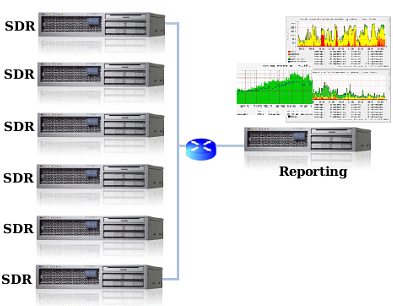
\includegraphics[width=80mm,height=60mm]{sdr-schema1.png}
\caption{SDR Recording/Reporting}
\label{fig:sdr-schema1}
\end{figure}

\bigskip
\noindent
There are four main recorders: sysrec, cpurec, nicrec, diskrec. 
Each recorder runs as a separate Perl5 process without any relation 
to the others. This makes very flexible to operation mode of all recorders, 
since they are autonomous. Additional there are different other recorders 
which can collect other type of system or application data: 
netrec, jvmrec, hdwrec, webrec. 

\noindent
All recorded data is stored as plain ASCII data, easy to be accessed by any 
3rd party system or other applications. The main idea is to have the data 
collection process standard between operating systems: Solaris, Linux, BSD. 

\bigskip
\noindent
The second module of SDR, the Reporting module, consists of several key
technologies: Round Robin Database Tool RRDtool, Perl 5, R Statistical Language, 
PDQ analytical solver all running on top of a HTTP server. All these coupled
with some visualization utilities makes SDR Reporting easy to be used in 
understanding the workloads running on a certain hardware infrastructure.

\endinput


% Recording Module
\chapter{Recording}
\noindent
Data recording module contains several operating system and
application related recorders. The current chapter will describe
what and how SDR recorders are functioning and how the recorded data
is delivered for analysis.

\section{Design}
A computer system has four main resources what will require monitoring:
CPU, Memory, Disks and Network devices. Such way SDR delivers 
four main recorders responsible to store system: cpu, memory, disk 
and network overall performance metrics over long periods of time 
saved on commodity storage, disks or SSDs. Additional specialized recorders, 
like Java Virtual Machine, process or network protocol statistics make 
SDR a complete recording system suitable for many types of computer systems.

\subsection*{Time series}
To keep things simple SDR is making available all collected metrics as variable
measured sequentially in time, called time series. All these observations
collected over fixed sampling intervals create a historical time series. 
To easy the access to all this set of data SDR simple records and stores 
the observations on commodity disk drives, compressed, in text format.

Time series let us understand what has happened in past and look in the future,
using various statistical models. In addition , having access to these 
historical time series will help us to build a simple capacity planning model 
for our application or site.

\subsection*{Raw Data}
All recorded observations we call them raw data. This set of data is not 
modified, altered or changed in any way and it is entirely the way we 
collected from the computer system. Its format is simple, as already 
mentioned, having its parameters collected : separated. Each recorder will 
write and store all collected parameters under such raw data file for the 
entire duration of its execution. By default, the SDR raw data extension 
is named, sdrd, system data recorder datafile.


\subsection*{Recorders}
The recording process consists of a number of running recorders, 
light probes developed in a dynamic language like Perl5 which can directly
talk and extract from operating system interfaces, the parameters we are
interested in. For example on Linux based systems we directly extract
various metrics from /proc interface. On Solaris systems we interact with
KSTAT interface to record all needed parameters.

Each recorder should be capable of accessing operating system
interfaces without calling additional utilities and display its data in
the following manner:

\begin{center}
\small{
timestamp:metric1:metric2:...:metricN \\
timestamp:metric1:metric2:...:metricN}
\end{center}

, where timestamp is defined as UNIX time or POSIX time and metricN
are the values collected from OS or application.

Typical a computer system will have deployed four standard recorders,
sysrec, cpurec, nicrec, diskrec along with additional specialized
recorders for different other purposes: network protocol statistics,
like TCP, UDP or IP represented by netrec, along with jvmrec or
procrec, webrec, zonerec. Below a complete list of all currently
supported recorders:

\begin{enumerate}
\item sysrec: overall system cpu, mem, disk and net utilization
\item cpurec: per-cpu statistics
\item nicrec: per-NIC statistics
\item diskrec: per-disk drive statistics
\item corerec: SPARC CMT T1, T2 processor statistics
\item netrec: UDP, IP, TCP/IP statistics
\item hdwrec: hardware, software inventory
\item jvmrec: Java Virtual Machine Garbage Collector statistics
\item procrec: per-process statistics
\item webrec: HTTP response time statistics
\item zonerec: Solaris zone statistics
\end{enumerate}

Certain monitoring systems use the concept of agentless recording, 
a system which runs on a centralized machine and executes via 
SSH or RSH operating system commands or custom probes on a number 
of hosts returning the results. Example here: HP SiteScope.

SDR uses by default a number of recorders on each monitored host,
therefore uses a agent based type. 

\subsection*{Transport Modes}
All observations are recorded for a number of days on each computer system. 
However we would like to send this data to a reporting backend where we could 
do some analysis and see it in a visual way. There are currently two ways 
to transport sdrd raw data for analysis: instant and batch modes.

\begin{enumerate}
\item Instant Mode\\
First mode of transporting the raw data to a reporting backend system 
is the instant mode. On this mode, the output of each data recorder will be 
scanned by a special utility, sender responsible to detect each changes 
and send over a SSH2 channel this data for analysis. Sender will scan 
periodically all sdrd raw data files, configured under a XML type of 
configuration and it will send these changes, secure to the reporting 
backend. This way we ensure each recorded data will arrive for analysis 
as soon as it has happened.

\item Batch Mode\\
The other mode, where we would like to see changes less often, like every 
24 hrs, would mean we will transport each sdrd raw data every 24 hrs to 
a reporting backend system for analysis using raw2day utility. This 
utility simple transports all recorded sdrd data for 1 day using SSH2 or FTP.
\end{enumerate}


% Configuration
\section{Configuration}
SDR Recording and Reporting modules use a XML based configuration
file to store its settings. This section describes the sdr.conf
for both recording and reporting modules.

Recorders, do not use sdr.conf, to minimize memory consumption and load
as few as possible different Perl5 modules.

\begin{center}
\begin{minipage}{0.9\textwidth}
\lstset{language=XML}
\begin{lstlisting}
<?xml version="1.0" encoding="UTF-8"?>
<sdr>
  <recording description="SDR Recording Module Configuration">

    <!-- Default Path -->
    <base_log path="/opt/sdr/log" description="Base log directory" />
    <current_log path="/opt/sdr/log/current" description="Current log directory" />
    <daily_log path="/opt/sdr/log/daily" description="Daily log directory" />

    <!-- SSH Public Key -->
    <private_key path="" description="The private authentication key" />

    <!-- Instant Monitoring -->
    <sender description="Sender configuration">
      <sdrd name="sys"  description="Overall system sysrec.sdrd"  />
      <sdrd name="cpu"  description="CPU cpurec.sdrd"  />
      <sdrd name="disk" description="Disk diskrec.sdrd" />
      <sdrd name="nic"  description="NIC nicrec.sdrd"  />
    </sender>

  </recording>

  <reporting description="SDR Reporting Module Configuration">

    <!-- Generic DB and Docroot settings -->
    <db path="/opt/sdr/report/db" description="SDR Reporting DB"/>
    <docroot path="/opt/sdr/report/docroot" description="SDR Reporting Docroot"/>

    <!-- Destination Reporting Servers -->
    <host name="reporting" ver="0.74" description="SDR Reporting Server">
      <username>sdr</username>
      <!-- PLEASE USE SSH Public Key Based Authentication ! -->
      <password></password>
    </host>

  </reporting>
</sdr>
\end{lstlisting}
\end{minipage}
\end{center}

There are two utilities using the main configuration file,
sdr.conf: raw2day and sender.  Below you can see a short description
of each element and attribute used by sdr.conf regarding recording module.

\begin{center}
\rowcolors{2}{gray!25}{white}
 \begin{tabular}{ccc}
 \rowcolor{gray!25}
  \textbf{Element} & \textbf{Values} & \textbf{Description} \\
  \small{base\_log}    & \small{path="/opt/sdr/log"}         & \small{Base log directory} \\
  \small{current\_log} & \small{path="/opt/sdr/log/current"} & \small{Current log directory} \\
  \small{daily\_log}   & \small{path="/opt/sdr/log/daily"}   & \small{Daily log directory} \\
  \small{private\_key} & \small{path=""} & \small{The private authentication key} \\
  \small{sender} & ~ & \small{Instant Monitoring} \\
  \small{sdrd} & \small{name="sys"}  & \small{Overall system sysrec.sdrd} \\
  \small{sdrd} & \small{name="cpu"}  & \small{CPU cpurec.sdrd} \\
  \small{sdrd} & \small{name="disk"} & \small{Disk diskrec.sdrd} \\
  \small{sdrd} & \small{name="nic"} & \small{NIC nicrec.sdrd} \\
\end{tabular}
\end{center}


\section{Standard System Recorders}
These are the main, basic recorders responsible for CPU, Mem, Disk
and Network utilization. These recorders must be active under any
system you plan to record data from.



% SYSREC
\subsection*{sysrec}
Records overall system statistics. Uses Perl5 and it is available for 
Linux and Solaris based operating systems. sysrec records system 
performance metrics: cpu, memory utilization, disk and network throughput, 
errors and system load averages. The recorder reports several key metrics 
across all devices, being the main recorder of SDR, responsible for 
overall system performance. This  will be the first place to check how your 
system performs in the long run.


\subsubsection{Linux}

%\rowcolors{2}{gray!25}{white}
%\begin{tabular}{cc}
%\rowcolor{gray!25}\small
%Metrics & 26 \\
%Kernel  & 2.6 32/64bit \\
%OS & RHEL 5.x \\
% & Ubuntu Server Edition \\
%\end{tabular}

The recorder uses Sys::Statistics::Linux to fetch all metrics. sysrec records 
up to 39 Linux OS parameters on x64 and x86 platforms ! sysrec supports two
operating modes: the default and the extended mode. The difference is that 
when sysrec runs under extended mode the memory figures will be detailed 
reported ! The raw data is already prepared and formatted for SDR analysis 
process. The recorder runs continuously.

This recorder supports interval values lower than second ! Running the
recorder with values lower than second for long periods of
time will add an overhead in terms of CPU utilization. The lower
the interval value the higher the CPU utilization. We do not
recommend using values lower than second for long historical recordings !

\begin{figure}[!ht]
\centering
% includegraphics[width=160mm,height=60mm]{sysrec_linux.png}
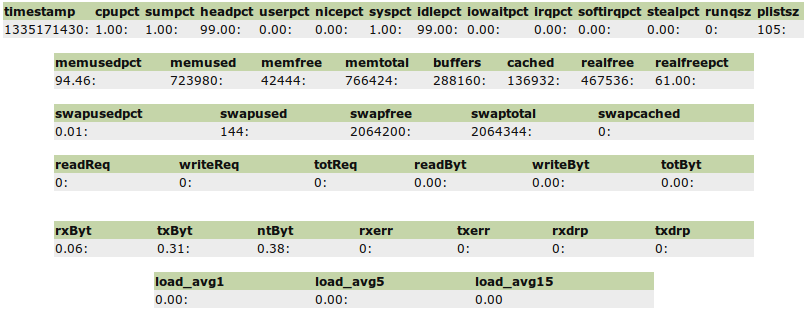
\includegraphics[scale=0.62]{sysrec_linux.png}
\caption{sysrec Linux}
\label{fig:sysrec.linux}
\end{figure}


\noindent
sysrec records system utilization along with certain other important metrics:
\begin{verbatim}
  CPU
   #01 timestamp  : seconds since Epoch
   #02 cpupct     : CPU Utilization, across all CPUs, percentage, gauge
   #03 sumpct     : sum of all CPUs Utilization, percentage, gauge
   #04 headpct    : headroom CPU available, all CPUs, percentage, gauge
   #05 userpct    : CPU Utilization User space in percent, gauge
   #06 nicepct    : CPU Utilization User space with nice priority, gauge
   #07 sysct      : CPU Utilization System space, gauge
   #08 idlepct    : CPU Utilization Idle state, gauge
   #09 iowaitcpt  : CPU Percentage in Idle state because an I/O, gauge
                    operation is waiting to complete, gauge
   #10 irqpct     : CPU Percentage servicing interrupts, gauge
   #11 softirqpct : CPU Percentage servicing softirqs, gauge
   #12 stealpct   : CPU Percentage of time spent in other operating systems
                    when running in a virtualized environment, gauge
   #13 runqsz     : run queue length, number of tasks waiting for run time
   #14 plistsz    : number of tasks in the task list

  MEM
   #15 memusedpct : size of used memory in percent, gauge
   #16 memused    : size of used memory in kilobytes, gauge (ext)
   #17 memfree    : size of free memory in kilobytes, gauge (ext)
   #18 memtotal   : size of memory in kilobytes, gauge (ext)
   #19 buffers    : size of buffers used from memory in kilobytes, gauge (ext)
   #20 cached     : size of cached memory in kilobytes, gauge (ext)
   #21 realfree   : size of memory is real free, gauge 
                     (memfree+buffers+cached) (ext)
   #22 realfreepct: size of memory is real free in percent of total memory,
                     gauge (ext)
   #23 swapusedpct: size of used swap space in percent, gauge
   #24 swapused   : size of swap space is used is kilobytes, gauge (ext)
   #25 swapfree   : size of swap space is free in kilobytes, gauge (ext)
   #26 swaptotal  : size of swap space in kilobytes, gauge (ext)
   #27 swapcached : memory that once was swapped out, is swapped back in 
                     but still also is in the swapfile, gauge (ext)

  DISK
   #28 readReq    : disk read requests, gauge
   #29 writeReq   : disk write requests, gauge
   #30 totReq     : disk read+write requests, gauge
   #31 readByt    : read bytes / sec, in KB, gauge
   #32 writeByt   : write bytes / sec, in KB, gauge
   #33 totByt     : read+write bytes / sec, in KB, gauge

  NET
   #34 rxByt      : received bytes /sec, in KB, gauge
   #35 txByt      : transmitted bytes /sec, in KB, gauge
   #36 ntByt      : received + transmitted bytes /sec, in KB, gauge
   #37 rxerr      : No. of errors that happend while received pckt/second
   #38 txerr      : No. of errors that happend while transmitting pckt/second
   #39 rxdrp      : No. of rx packets that were dropped per second
   #40 txdrp      : No. of tx packets that were dropped per second
 
   #41 avg_1      : LA of the last minute
   #42 avg_5      : LA of the last 5 minutes
   #43 avg_15     : LA of the last 15 minutes
\end{verbatim}


\subsubsection{Solaris}
sysrec on Solaris is a utility, part of K9Toolkit, author Brendan Gregg. 
The toolkit is a collection of free Perl scripts used to troubleshoot and 
observe Solaris systems. sysrec records 14 Solaris OS metrics on x64 and
sparcv9 platforms. The recorder has been modified to output its data as RRD.

\begin{figure}[!ht]
\centering
%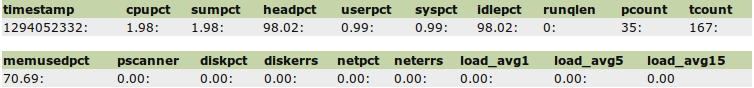
\includegraphics[width=145mm,height=15mm]{sysrec_sol.png}
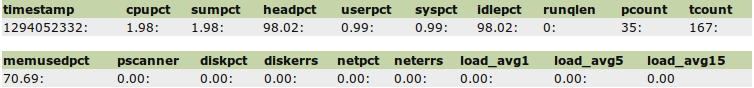
\includegraphics[scale=0.62]{sysrec_sol.png}
\caption{sysrec Solaris}
\label{fig:sysrec.linux}
\end{figure}

sysrec records system utilization and certain additional kernel statistics
used as a starting point in observing the system's general health. The output
from sysrec is displayed below:

\begin{verbatim}
  CPU
   #01 timestamp  : seconds since Epoch
   #02 cpupct     : CPU Utilization, across all CPUs, percentage, gauge
   #03 sumpct     : sum of all CPUs utilization, percentage, gauge
   #04 headpct    : headroom CPU available, all CPUs, percentage, gauge
   #05 userpct    : CPU Utilization User space, all cpus, percentage, gauge
   #06 syspct     : CPU Utilization System space, all cpus, percentage, gauge
   #07 idlepct    : CPU Utilization Idle state, all cpus, percentage, gauge
   #08 runqlen    : threads on the run queue, gauge
   #09 pcount     : current process count on the system
   #10 tcount     : current lwp count on the system

  MEM
   #11 memusedpct : size of used memory in percent, gauge
   #12 pscanner   : scan rate of the page scanner, gauge
 
  DISK
   #13 diskpct    : sum read+write across disks, percentage, gauge
   #14 diskerrs   : operations on the wait queue, gauge

  NET
   #15 netpct     : throughput, read+write bytes across NICs, percentage, gauge
   #16 neterrs    : number of errors due to buffer saturation

   #17 la_1       : Load Average 1min
   #18 la_5       : Load Average 5min
   #19 la_15      : Load Average 15min
\end{verbatim}


\noindent
\newline
Examples for Linux and Solaris operating systems:



\begin{center}
\begin{tabular}{lll}

\multicolumn{3}{c}{} \\
\textbf{Mode} & \textbf{Example} & \textbf{Description} \\ \hline
\newline

\multirow{4}{*}{\small{Default Mode}} & 
 \small{\emph{sysrec}} & \small{print summary since boot only}\\ & 
 \small{\emph{sysrec 60}} & \small{print every 60secs system stats}\\ & 
 \small{\emph{sysrec 1 5}} & \small{print 5 times, every 1secs system stats}\\ &
 \small{\emph{sysrec .5}} & \small{print every 0.5secs system stats}\\
 \hline

\multirow{2}{*}{\small{Extended Mode}} & 
 \small{} & \small{Linux Only} \\ &
 \small{\emph{sysrec -x 5}} & \small{print every 5secs extended 
    system stats, detailed memory figures}

\end{tabular}
\end{center}



% CPUREC
\subsection*{cpurec}
Records per CPU parameters from a Linux or Solaris system. On a multiprocessor
environment cpurec will display all CPUs and all parameters associated with them.

\subsubsection{Linux}
The recorder uses Sys::Statistics::Linux Perl module to extract and compute
all CPU statistics. cpurec records 10 Linux OS metrics on x64 and x86 platforms !
The recorder has been modified to output its data as RRD.  

\begin{figure}[!ht]
\centering
%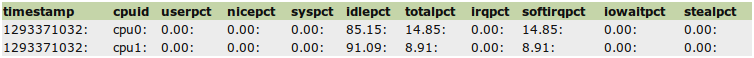
\includegraphics[width=145mm,height=12mm]{cpurec_lin.png}
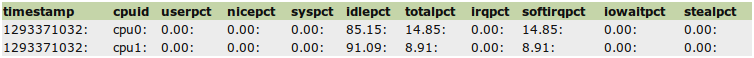
\includegraphics[scale=0.62]{cpurec_lin.png}
\caption{cpurec Linux}
\label{fig:cpurec_lin}
\end{figure}

\noindent
cpurec records system utilization along with certain other important metrics:

\begin{verbatim}
  #01 timestamp  : seconds since Epoch
  #02 cpuid      : CPU id
  #03 user       : CPU Utilisation User space percentage, gauge
  #04 nice       : CPU utilisation User space nice priority percentage, gauge
  #05 system     : CPU utilisation System space percentage, gauge
  #06 idle       : CPU Utilisation idle state percentage, gauge
  #07 total      : Total CPU Utilisation percentage, gauge
  #08 irq        : CPU Percentage servicing interrupts, gauge
  #09 softirq    : CPU Percentage servicing softirqs, gauge
  #10 iowait     : CPU Percentage in idle state because an I/O 
                    operation is waiting to complete, gauge
  #11 steal      : CPU Percentage of time spent in other operating systems 
                    when running in a virtualized environment, gauge
\end{verbatim}


\subsubsection{Solaris}
cpurec is a utility, collecting per-CPU data from kstat. The recorder outputs
its data under RRD format. cpurec records 12 Solaris OS metrics on x64 and
sparcv9 platforms !  cpurec used mainly to observe CPU activity and
analyse how the CPUs are used in the system. Useful for capacity planning.

\begin{figure}[!ht]
\centering
%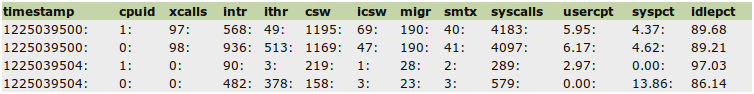
\includegraphics[width=145mm,height=18mm]{cpurec_sol.png}
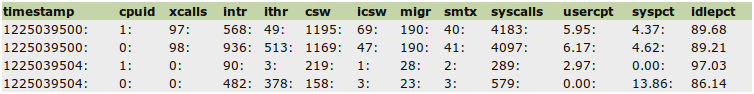
\includegraphics[scale=0.62]{cpurec_sol.png}
\caption{cpurec Solaris}
\label{fig:cpurec_sol}
\end{figure}

\noindent
Recording parameters:

\begin{verbatim}
  #01 timestamp: seconds since Epoch
  #02 Xcalls   : rate of multiprocessor cross calls, gauge
  #03 Intr     : rate of intrerrupts, gauge
  #04 iThr     : rate of interrupts threads, gauge
  #05 Csw      : rate of context switches, gauge
  #06 Icsw     : rate of involuntary context switches, gauge
  #07 Migr     : rate of migrations, gauge
  #08 Smtx     : rate of kernel mutexes, gauge
  #09 Syscalls : rate of system calls, gauge
  #10 User     : percentage of time spent in user mode, gauge
  #11 Sys      : percentage of time spent in sys mode, gauge
  #12 Idle     : percentage of time spent in idle mode, gauge
\end{verbatim}


\noindent
\newline
Examples for Linux and Solaris operating systems:


\begin{center}
\begin{tabular}{lll}
\multicolumn{3}{c}{} \\
\textbf{Mode} & \textbf{Example} & \textbf{Description} \\ \hline
\newline

\multirow{4}{*}{\small{Default Mode}} &
 \small{\emph{cpurec}} & \small{print summary since boot only}\\ &
 \small{\emph{cpurec 60}} & \small{print every 60secs per CPU stats}\\ &
 \small{\emph{cpurec 1 5}} & \small{print 5 times, every 1secs per CPU stats}\\ &
 \small{\emph{cpurec .5}} & \small{print every 0.5secs per CPU stats}\\
% \hline

%\multirow{1}{*}{\small{Extended Mode}} &
% \small{} & \small{} \\ &
% \small{\emph{sysrec -x 5}} & \small{print every 5secs extended
%    system stats, detailed memory figures}

\end{tabular}
\end{center}



%\subsection*{diskrec}
%Not yet available !



% NICREC
\subsection*{nicrec}
nicrec records per NIC statistics. Useful to measure the throughput of one
or many network cards or the number of errors during transmitting or receiving 
packets.

\subsubsection{Linux}
The recorder uses Sys::Statistics::Linux to fetch all metrics. nicrec records
19 Linux OS metrics on x64 and x86 platforms ! The recorder has been modified 
to output its data as RRD and no delta values are stored, but rather raw data.

\begin{figure}[!ht]
\centering
%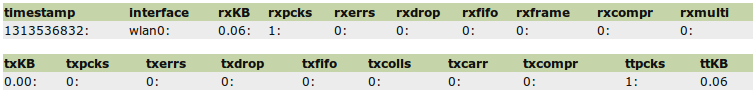
\includegraphics[width=145mm,height=18mm]{nicrec_lin.png}
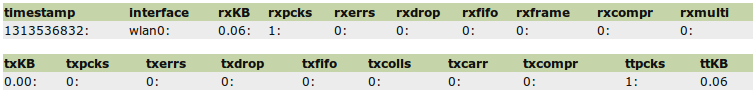
\includegraphics[scale=0.62]{nicrec_lin.png}
\caption{nicrec Linux}
\label{fig:nicrec_lin}
\end{figure}

\noindent
nicrec records per NIC metrics: 

\begin{verbatim}
  #01 timestamp  : seconds since Epoch
  #02 interface  : the interface name, NIC name
  #03 rxKB       : the no. of KBytes received/sec, gauge
  #04 rxpcks     : the no. of packets received/sec, gauge
  #05 rxerrs     : the no. of errors while received packets/sec, gauge
  #06 rxdrop     : the no. of packets that were dropped/sec, gauge
  #07 rxfifo     : the no. of FIFO overruns on received packets/sec, gauge
  #08 rxframe    : the no. of carrier errors on received packets/sec, gauge
  #09 rxcompr    : the no. of compressed packets received/sec, gauge
  #10 rxmulti    : the no. of multicast packets received/sec, gauge
  #11 txKB       : the no. of KBytes transmitted/sec, gauge
  #12 txpcks     : the no. of packets transmitted/sec, gauge
  #13 txerrs     : the no. of errors transmitting packets/sec, gauge
  #14 txdrop     : the no. of packets that were dropped/sec, gauge
  #15 txfifo     : the no. of FIFO overruns on transmitted packets/sec, gauge
  #16 txcolls    : the no. of collisions that were detected/sec, gauge
  #17 txcarr     : the no. of carrier errors on transmitted packets/sec, gauge
  #18 txcompr    : the no. of compressed packets transmitted/sec, gauge
  #19 ttpcks     : the no. of total packets (received + transmitted)/sec, gauge
  #20 ttKB       : the no. of total KBytes (received + transmitted)/sec, gauge
\end{verbatim}


\subsubsection{Solaris}
nicrec is a utility part of K9toolkit, author Brendan Gregg, printing network
traffic, KB/s transferred per network interface, packet counts and average
sizes. nicrec records 9 Solaris OS metrics on x64 and sparcv9 platforms ! 
The recorder outputs its data under RRD format.

\begin{figure}[!ht]
\centering
%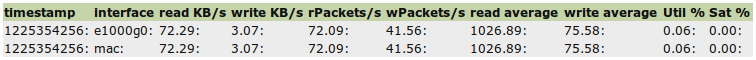
\includegraphics[width=145mm,height=12mm]{nicrec_sol.png}
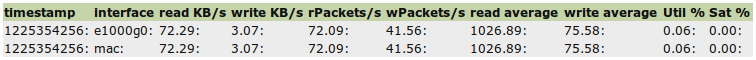
\includegraphics[scale=0.62]{nicrec_sol.png}
\caption{nicrec Solaris}
\label{fig:nicrec_sol}
\end{figure} 

\noindent
Recording parameters:
\begin{verbatim}
  #01 timestamp: seconds since Epoch
  #02 int      : interface
  #03 rKB/s    : read KB/s, gauge
  #04 wKB/s    : write KB/s, gauge
  #05 rPk/s    : read Packets/s, gauge
  #06 wPk/s    : write Packets/s, gauge
  #07 rAvs     : read Average size, bytes
  #08 wAvs     : write Average size, bytes
  #09 %Util    : utilisation (read+write)/nic speed, gauge
  #10 Sat      : Saturation: defer, nocanput, norecvbuf, noxmtbuf, gauge
\end{verbatim}

\noindent
\newline
Examples for Linux and Solaris operating systems:

\begin{center}
\begin{tabular}{lll}
\multicolumn{3}{c}{} \\
\textbf{Mode} & \textbf{Example} & \textbf{Description} \\ \hline
\newline

\multirow{4}{*}{\small{Default Mode}} &
 \small{\emph{nicrec}} & \small{print summary since boot only}\\ &
 \small{\emph{nicrec 60}} & \small{print every 60secs per NIC stats}\\ &
 \small{\emph{nicrec 1 5}} & \small{print 5 times, every 1secs per NIC stats}\\ &
 \small{\emph{nicrec .5}} & \small{print every 0.5secs per NIC stats}\\
% \hline

%\multirow{1}{*}{\small{Extended Mode}} &
% \small{} & \small{Linux Only} \\ &
% \small{\emph{sysrec -x 5}} & \small{print every 5secs extended
%    system stats, detailed memory figures}

\end{tabular}
\end{center}


\section{Specialized Recorders}
These are recorders specific for different applications or certain
parts of the operating system only. These are optional recorders and
should be enabled only on systems which require such monitoring.


% COREREC
\subsection*{corerec}
A SPARC processor specific recorder, responsible to report per core
utilization. This is a Solaris/SPARC system recorder only !

\subsubsection{Solaris}
corerec is a utility using corestat, from Cooltools, original project of
Sun Microsystems Inc. The output is not formatted for SDR Reporting module 
and it is simple as human readable format.

corerec is used to observe core utilization from a T1 or T2 processor. Since T1
and T2 have different registers for keeping track of the usage the corestat
utility has to be different for each case: corestat.t1 used for T1 processors
and corestat.t2 for T2. 

\noindent
Recording parameters:

\begin{verbatim}
%Usr: percentage user time
%Sys: percentage sys time
%Usr+Sys: both Usr + Sys
Avg: core utilization

The output from corerec is displayed below:

For a T2 processor:
Core,Int-pipe     %Usr     %Sys     %Usr+Sys 
    0,0           0.05      0.37      0.42 
    0,1           0.06      0.07      0.13 
    1,0           0.04      0.08      0.12 
    1,1           0.01      0.05      0.06 
    2,0           0.09      0.11      0.20 
    2,1           0.01      0.06      0.07 
    3,0           0.02      0.15      0.17 
    3,1           0.01      0.05      0.05 
    4,0           0.01      0.13      0.14 
    4,1           0.01      0.04      0.05 
    5,0           0.07      0.10      0.16 
    5,1           0.01      0.45      0.46 
    6,0           0.02      0.10      0.12 
    6,1           0.01      0.06      0.07 
    7,0           0.03      0.12      0.14 
    7,1           0.05      0.06      0.01 
-------------     -----     -----    ------ 
    Avg           0.03      0.12      0.15 

\end{verbatim}

Important to note here is that utilization for a T1 or T2 processor does not
simple mean data from vmstat, mpstat or sysrec, cpurecalone. You have to use 
corerec in order to gather the per core utilization figures. 



% JVMREC
\subsection*{jvmrec}
jvmrec records per JVM garbage collection statistics. It is very important to
understand and check how well your Java applications are running. For this we
will need to look and check internal Java Virtual Machine parameters, 
like the garbage collection statistics. The recorders uses jstat, part of 
standard JDK displaying its data under RRD format.


\subsubsection{Linux}
jvmrec records the GC statistics useful to understand how your JVMs are
running. jvmrec can easily filter certain JVMs using -f format option 
, where format is a Perl regexp. The format is used mainly to filter,
search over a number of running JVMs for a specific set and use only 
those ! jvmrec as well supports an extended mode, when used the utility 
will report Disk IO statistics along with GC activity. This is useful 
in cases a Java application is heavily GCing and it does create a lot of
Disk IO.

\noindent
Recording parameters:

\begin{verbatim}
  #01 timestamp  : seconds since Epoch
  #02 name.pid   : JVM name and process ID
  #03 S0         : Survivor S0 utilisation, percentage, gauge
  #04 S1         : Survivor S1 utilisation, percentage, gauge
  #05 Eden       : Eden space utilisation, percentage, gauge
  #06 Old        : Old space utilisation, percentage, gauge
  #07 Perm       : Permanent space utilisation, percentage, gauge
  #08 No.mGC     : Number of young generation GC events
  #09 Time.mGC   : Young generation garbage collection time, secs
  #10 No.MGC     : Number of full GC events
  #11 Time.MGC   : Full garbage collection time, secs
  #12 TotalGC    : Total garbage collection time, secs
  #13 utime      : The no. of jiffies scheduled in user mode
  #14 stime      : The no. of jiffies scheduled in kernel mode
  #15 size       : The total program size of the process
  #16 resident   : The resident set size, the text, data and stack space
  #17 nswap      : The size of swap space of the proces
  #18 syscr      : Number of read syscalls
  #19 rchar      : Bytes read from storage (might have been from pagecache)
  #20 read_bytes : Bytes really fetched from storage layer
  #21 syscw      : Numner of write syscalls
  #22 wchar      : Bytes written
  #23 write_bytes: Bytes sent to the storage layer
\end{verbatim}


\subsubsection{Solaris}
jvmrec records GC statistics useful to understand how your JVMs are
running. jvmrec is implemented as a KSH recorder on Solaris.

\noindent
Recording parameters:

\begin{verbatim}
  #01 timestamp : seconds since Epoch
  #02 zone.pid  : name of the zone and process ID
  #03 S0%       : Survivor S0 utilisation, percentage, gauge
  #04 S1%       : Survivor S1 utilisation, percentage, gauge
  #05 Eden%     : Eden space utilisation, percentage, gauge
  #06 Old%      : Old space utilisation, percentage, gauge
  #07 Perm%     : Permanent space utilisation, percentage, gauge
  #08 No.mGC    : Number of young generation GC events
  #09 Time.mGC  : Young generation garbage collection time, secs
  #10 No.MGC    : Number of full GC events
  #11 Time.MGC  : Full garbage collection time, secs
  #12 TotalGC   : Total garbage collection time, secs
\end{verbatim}

\noindent
\newline
Examples for Linux and Solaris operating systems:
\begin{center}
\begin{tabular}{lll}

\multicolumn{3}{c}{} \\
\textbf{Mode} & \textbf{Example} & \textbf{Description} \\ \hline
\newline

\multirow{2}{*}{\small{Default Mode}} & \small{\emph{jvmrec 60}} &
 \small{print every 60secs stats all JVMs}\\

 & \small{\emph{jvmrec 5 10}} & \small{print every 5secs JVM stats 10
samples}\\
 \hline

\multirow{3}{*}{\small{Filter Mode}} &
 \small{\emph{jvmrec -f weblogic 60}} &
 \small{print every 60secs Weblogic stats}\\

 & \small{\emph{jvmrec -f '-Dmyapp.Name' 60}} &
   \small{print every 60secs all Dmyapp.Name JVMs}\\

 & \small{\emph{jvmrec -f '\^{}(?!.*?esite).*' 60}} &
   \small{print every 60secs all JVMs which are not called esite}\\

\hline
\multirow{2}{*}{\small{Extended Mode}} &
 \small{} & \small{Linux Only} \\ &
 \small{\emph{jvmrec -xf 'com*' 360}} &
 \small{print every 360secs all com JVMs including extended statistics}\\

\end{tabular}
\end{center}




% NETREC
\subsection*{netrec}
netrec records per protocol statistics: TCP, UDP for example. It does use an 
extra operating system utility, netstat. The recorder outputs its data under 
RRD format.

\subsubsection{Linux}
netrec records per protocol statistics TCP, UDP from netstat utility. The 
recorder uses netstat binary, so this utulity should be present on your Linux
installation. The recorder has been modified to output its data as RRD and no
delta values are stored, but rather raw data.

\begin{figure}[!ht]
\centering
%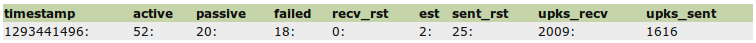
\includegraphics[width=145mm,height=9mm]{netrec_lin.png}
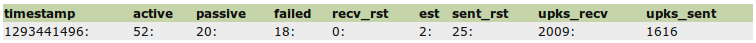
\includegraphics[scale=0.62]{netrec_lin.png}
\caption{netrec Linux}
\label{fig:netrec_lin}
\end{figure}

\noindent
Recording parameters:

\begin{verbatim}
  #01 timestamp  : seconds since Epoch
  #02 active     : TCP active connections, counter
  #03 passive    : TCP passive connections, counter
  #04 failed     : TCP failed connection attempts, counter
  #05 recv_rst   : TCP connection resets received, counter
  #06 est        : TCP connections established, gauge
  #07 sent_rst   : TCP resets sent, counter
  #08 upks_recv  : UDP packets received, counter
  #09 upks_sent  : UDP packets sent, counter
  #10 fast_retr  : Fast retransmits, counter
  #11 fwd_retr   : Forward retransmits, counter
  #12 slow_retr  : Retransmits in slow start, counter
\end{verbatim}




\subsubsection{Solaris}
netrec is a utility, reporting TCP, UDP and IP statistics from a running local
or global zone. If the system deploys one or more zones and if all zones share
same TCP/IP stack then you can simple use -s flag to report the numbers just
once. The recorder outputs its data under RRD format and no delta are stored !

\noindent
Recording parameters:

\begin{verbatim}
  #01 timestamp       : seconds since Epoch
  #02 zonename        : Solaris zone name
  #03 udpInDatagrams  : No. of UDP input datagrams
  #04 udpInErr        : No. of UDP input errors
  #05 udpOutDatagrams : No. of UDP output datagrams
  #06 udpOutErrors    : No. of UDP output errors
  #07 tcpActiveOpens  : No. of outgoing connections since boot, counter
  #08 tcpPassiveOpens : No. of incoming connections since boot, counter
  #09 tcpAttemptFails : No. of outgoing failures since boot, counter
  #10 tcpEstabResets  : No. of resets to terminate established connections
  #11 tcpCurrEstab    : No. of current established connections
  #12 tcpOutSegs      : Total no. of segments sent, counter
  #13 tcpOutDataSegs  : Sender total no. of data segments sent, counter
  #14 tcpOutDataBytes : Sender total no. of bytes in data segments sent,
                         counter
  #15 tcpRetransSegs  : Total no. of segments retransmitted
  #16 tcpRetransBytes : Sender total no. of bytes in segments retransmitted,
                         counter
  #17 tcpOutRsts      : No. of segments sent with RST flag, counter

  #18 tcpListenDrop   : Total no. of connections refused, backlog full
  #19 tcpListenDropQ0 : Total no. of connections refused, half-open queue full
  #20 tcpHalfOpenDrop : Total no. of connections dropped, full half-open queue
  #21 tcpOutSackRetrs : Total no. of retransmitted segments by SACK retrans
  #22 ipInHdrErr      : No. of dg discards for iph error
  #23 ipInAddrErr     : No. of dg discards for bad addr
  #24 ipInCksumErr    : No. of bad IP header checksum
  #25 tcpInErr        : Total no. of segments recv with error, counter
  #26 udpInCksumErr   : No. of UDP packets with bad UDP checksum, counter
\end{verbatim}



% PROCREC
\subsection*{procrec}
This is a Linux specific recorder. procrec records per process statistics: 
owner, state, nice, the priority of the process, the no. of light weight 
processes, the no. of open file descriptors, the no. of minor and major faults 
the process made and many other metrics. The recorder uses 
Sys::Statistics::Linux to fetch all metrics. The recorder has been modified to 
output its data as RRD and no delta values are stored, but rather raw data. 

\begin{figure}[!ht]
\centering
%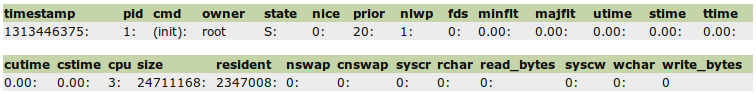
\includegraphics[width=145mm,height=20mm]{procrec_lin.png}
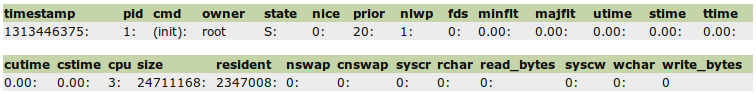
\includegraphics[scale=0.62]{procrec_lin.png}
\caption{procrec Linux}
\label{fig:procrec_lin}
\end{figure}

\noindent
Recording parameters:

\begin{verbatim}
  #01 timestamp  : seconds since Epoch
  #02 pid        : the process ID of the process
  #03 cmd        : command of the process
  #04 owner      : the owner of the process
  #05 state      : the status of the process
  #06 nice       : the nice level of the process
  #07 prior      : the priority of the process (+15)
  #08 nlwp       : the no. of light weight processes by this process
  #09 fds        : the no. of open file descriptors
  #10 minflt     : the no. of minor faults the process made
  #11 mayflt     : the no. of major faults the process made
  #12 utime      : the no. of jiffies proc have beed in user mode
  #13 stime      : the no. of jiffies proc have beed in kernel mode
  #14 ttime      : the no. of jiffies proc have beed (user + kernel)
  #15 cutime     : the no. of jiffies proc waited for childs in user mode
  #16 cstime     : the no. of jiffies proc waited for childs in kernel mode
  #17 cpu        : the CPU number the process was last executed on
  #18 size       : the total program size of the process, in bytes
  #19 resident   : the resident set size(the text, data, stack), in bytes
  #20 nswap      : the size of swap space of the process
  #21 cnswap     : the size of swap space of the childrens of the process
  #22 syscr      : number of read syscalls
  #23 rchar      : bytes read from storage (might have been from pagecache)
  #24 read_bytes : bytes really fetched from storage layer
  #25 syscw      : number of write syscalls
  #26 wchar      : bytes written
  #27 write_bytes: bytes sent to the storage layer
  #28 cmdline    : command line of the process (ext)
\end{verbatim}



% WEBREC
\subsection*{webrec}
This is a generic recorder, working under Linux or Solaris based
operating systems.  webrec is a utility based on Apache HTTPClient, 
written in Java intended to be used to measure response times for different 
HTTP actions: POST, GET. Currently webrec supports only GET HTTP methods. 
Work in under way to expand this to POST methods and authentication.

\begin{figure}[!ht]
\centering
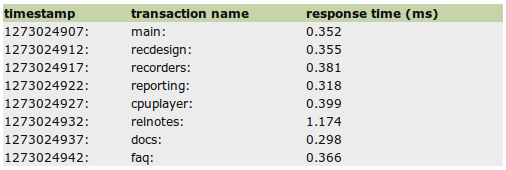
\includegraphics[width=105mm,height=35mm]{webrec.png}
\caption{webrec}
\label{fig:webrec}
\end{figure}

webrec checks for a master configuration file, called: webrec.conf located
under SDR/etc/ director, where SDR Recording module has been installed. It
parses the configuration file: webrec.conf and it retrieves the values for
timeout and the name definitions of each workload. For each workload it
creates a thread and its starting to follow each URL recording the response
times. WebRec supports Cookies as defined in RFC 2965 

webrec operates against one or many workloads. Workload defines a sequence of
URLs with the following properties:

\noindent
Recording parameters:

\begin{verbatim}
name    : name of the workload
delay   : delay after each URL (in seconds)
interval: the interval to invoke workloads (in seconds)
timeout : determines the timeout until a connection is
           etablished. A value of zero means the timeout is not used. The
           default value is zero. (in milliseconds)
\end{verbatim}



% ZONEREC
\subsection*{zonerec}
This is a Solaris only recorder, responsible to display per zone statistics. 
zonerec is a simple script calling prstat utility to report zone utilization in
human readable format. This data needs to be parsed and prepared in RRD
format. Future versions will include a new recorder which will output its data
to RRD format.

zonerec used to observe CPU and Mem utilization, as reported by prstat.



\begin{figure}[!ht]
\centering
%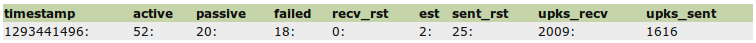
\includegraphics[width=145mm,height=9mm]{netrec_lin.png}
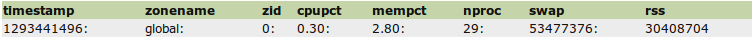
\includegraphics[scale=0.62]{zonerec_sol.png}
\caption{zonerec Solaris}
\label{fig:zonerec_sol}
\end{figure}

\noindent
Recording parameters:

\begin{verbatim}
  #01 timestamp: seconds since Epoch
  #02 zonename : Solaris zone name
  #03 zid      : Solaris zone id
  #04 cpu      : CPU utilisation, percentage, gauge
  #05 mem      : Mem utilisation, percentage, gauge
  #06 nproc    : no. of processes used by zoneid
  #07 swap     : total swap used by zoneid, includes tmpfs mounts, in bytes
  #08 rss      : resident set size, the amount of physical memory, in bytes
\end{verbatim}


% Transport Utilities
\section{Transport Utilities}
SDR Recording module contains some utilities to manage the recorded raw data: 
archive sdrd raw daily data, monitor and transport sdrd raw data changes 
to a reporting site for instant monitoring or transport archived data to a
reporting centralized site. For transport these tools use SSH2 or FTP protocols.

% RAW2DAY
\subsection*{raw2day}
raw2day is responsibile to create a compressed copy of the sdrd raw data, 
for the past day for archiving purposes. The utility, usually, operates in 
batch mode, at midnight, scheduled to run via crontab. By default the tool 
does not transport as well the data archived. To transport the archived data 
raw2day must be told to run the transport mode which supports SSH2 or FTP protocols.

\noindent
\newline
raw2day archives daily sdrd raw data and if neccesasrily transport it
to a dedicated reporting sserver:
\begin{verbatim}
USAGE: raw2day [-hV] [-t ftp|scp|sftp] [host...]
  e.g. raw2day               moves raw data to daily log
       raw2day -t ftp        switch transport to FTP
       raw2day -t sftp       switch transport to SFTP
       raw2day -t scp        switch transport to SCP
       raw2day -t sftp rep1  switch transport to SFTP and 
                              transport data to rep1 reporting server
NOTES:
   sdr.conf  : raw2day uses sdr.conf XML configuration file !
\end{verbatim}


\noindent
\newline
Examples for Linux and Solaris operating systems:

\begin{center}
\begin{tabular}{lll}

\multicolumn{3}{c}{} \\
\textbf{Mode} & \textbf{Example} & \textbf{Description} \\ \hline
\newline

\multirow{1}{*}{\small{Default Mode}} & 
 \small{\emph{raw2day}} & \small{archives daily sdrd raw data}\\
 \hline

\multirow{3}{*}{\small{Transport Mode}} & 
 \small{\emph{raw2day -t ftp}} & \small{archives daily sdrd raw data and transports it using FTP}\\ & 
 \small{\emph{raw2day -t sftp}} & \small{archives daily sdrd raw data and transports it using SFTP}\\ &
 \small{\emph{raw2day -t sftp rep1}} & \small{switch transport to SFTP and transport data to rep1 reporting server}
\end{tabular}
\end{center}

% RAW2DAY
\subsection*{sender}
sender  is  responsible  for sending sdrd raw data updates to a backend
reporting system for instant monitoring:  updates,  plotting.  It  uses
SSH2 for a secure transport between each recording host and the backend
reporting server.

During its start, sender, will look  for  the  main  SDR  configuration
file,  sdr.conf  to  fetch what sdrd raw data files will look after and
where to transport the changes. Make sure you  have  a  single  backend
reporting  server defined currently under sdr.conf ! Currently the last
definition of the reporting host will be used.

The utility uses SSH2 transport libraries to create a  connection  from
each  recording host to a backend reporting system and send all updates
via this connection. In case  of  a  temporarily  failure  sender  will
reopen the SSH2 connections and start sending the updates again. If for
some reasons the backend system wont answer in a  proper  time,  sender
will wait until the reporting will allow connections or comeback alive.
In case of a fatal connection failure sender will wait permanentely for
the backend reporting server.

By  default,  sender will output all its messages and errors under pre‐
fix/log/sender.log log file. For example the default installation will
have sender output all info and error messages under /opt/sdr/log/sender.log

\noindent
\newline
\begin{verbatim}
USAGE: sender [-t secs] [-hV] | [interval]
OPTIONS:
  -t        : timeout in seconds
  -h        : help information
  -V        : release version
  interval  : maximum number of seconds between samples, default 60, will 
              never spend more than that without checking data

 e.g. sender     check and send sdrd raw data, every 60 secs
      sender 10  check and send sdrd raw data, every 10 secs

NOTES:
 sdr.conf: sender uses sdr.conf XML configuration file ! Make sure you
 have a functional sdr.conf installed or define where sdr.conf
 is found using SDR_ROOT variable
\end{verbatim}



\endinput


%Reporting Module
\chapter{Reporting}

\noindent
One important part of SDR is the way we gather and aggregate all recorded data
from all our systems and finally compile simple reports. One major goal, when
designing the reporting module, was to be able to get all these things in
matter of minutes, saving your time in front of computer. As well, another 
important part was to be able to use different data visualization engines 
for all recorded data.

\section{Design}
By default, the reportign package uses RRDtool, the high performance data logging 
and graphing system as our performance database. We generate all reports, plots 
based on RRDtool.

However we are not restricted to RRDtool since we do have all raw data collected. 
We are using as well R statistical computing and graphics language for analysing 
all recorded data using heatmaps or treemaps representation. At last, we like 
to bring closely geometry and performance analysis: cuplayer, a visual player 
of multiprocessor data, cpurec, using Barycentric coordinates, which displays 
the CPU transition states from IDLE to USER or SYSTEM time.

\begin{figure}[!ht]
\centering
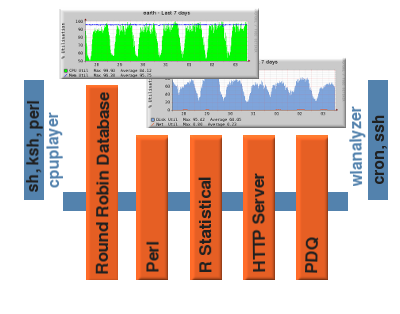
\includegraphics[width=75mm,height=55mm]{sdr-rep-schemaf.png}
\caption{SDR Reporting module}
\label{fig:sdr-rep-schemaf}
\end{figure}

This way, SDR Reporting contains several sub-modules, each with its own purpose:

\begin{enumerate}

\item Data visualization engine:\\
a standard component responsible for all plots and reports within SDR Reporting. 
This uses RRDtool, R, cpuplayer and Perl

\item Workload management engine:\\
includes different workload management tools for web and streaming based 
services: 
\begin{itemize}
 \item wlanalyzer: HTTP based workloads
 \item slanalyzer: RTMP, RTSP based workloads
\end{itemize}

\end{enumerate}

All these things make the reporting module simple and apart from other 
reporting systems:

\begin{itemize}
\item Not an analytics package
\item Simple pre-compiled reports, always work
\item Very simple to understand
\item Easy customizations
\item You don't have to click, dozens of options, links to get what you need
\item Should save your time in front of computer, being simple and to the point
\item Simple to educate your IT staff
\end{itemize}

\section{Configuration}


\endinput


% Installation
\chapter{Installation}
\noindent
This chapter lists the product requirements and the installation
notes for SDR.

% %%%%%%%%%%%%
% REQUIREMENTS
% %%%%%%%%%%%%
\section{Requirements}
\noindent
Before running SDR, make sure all product requirements
are satisfied by checking all your servers, where
you plan to install the software. SDR requires to be installed 
on each server you plan to collect data from and one additional 
server, where you plan to keep all recorded data, the reporting server.

\subsection*{Recording Module}
This modules contains the Perl5 environment, OpenSSL and some
additional libraries and all SDR recorders and utilities.

In addition, some Perl modules specific to certain operating systems are as well 
found under recording module, for example: Sun::Solaris::Kstat and
Linux::System::Statistics.

\begin{center}
\begin{tabular}{lll}

\multicolumn{3}{c}{} \\
 \rowcolor{blue!25}
 \textbf{Item} & \textbf{Minimum Requirement} & \textbf{Description} \\
 \hline
 \newline

\multirow{1}{*}{\small{Memory}} &
 \small{128MB RAM} & \small{standard and specialized recorders} \\
 \hline

\multirow{2}{*}{\small{Storage}} &
 \small{150MB} & \small{default installation: 150MB} \\ &
 \small{1MB} & \small{raw data: per day raw data, per host} \\
 \hline

\multirow{4}{*}{\small{Operating Systems}} &
 \small{} & \small{RedHat Entreprise Linux 5.x,6.x} \\ &
 \small{Linux 2.6+} & \small{Ubuntu Server 10.x,11,12+ LTS} \\ &
 \small{} & \small{Ubuntu Server 10.x,11,12+ LTS} \\ &
 \small{Solaris 10} & \small{Solaris 10 Update 6, x64, SPARC} \\
 \hline

\multirow{1}{*}{\small{System Libraries}} &
 \small{zlib} & \small{Linux based operating systems} \\
 \hline

\multirow{2}{*}{\small{Shell}} &
 \small{ksh93} & \small{Linux based operating systems} \\ &
 \small{ksh88} & \small{Solaris} \\
 \hline

\multirow{1}{*}{\small{Utilities}} &
 \small{chkconfig} & \small{Linux based operating systems} \\ &
 \small{cron} & \small{update-rc.d cron defaults} \\
 \hline

\multirow{1}{*}{\small{Java}} &
 \small{Java 6,7} & \small{Linux,Solaris} \\
 \hline

\multirow{1}{*}{\small{Virtualization}} &
 \small{SUNWzoner,SUNWzoneu} & \small{Solaris zones}

\end{tabular}
\end{center}



\subsection*{Reporting}
\noindent
These are the product requierements for SDR Reporting module for all supported
operating systems. RedHat/Ubuntu, Solaris SDR reporting module can be 
installed under RedHat/Ubuntu or Solaris based systems. Currently
the reporting module has been tested under Solaris 10 Update 8 x64 and
SPARC V9. SDR Reporting ships with its own Perl distribution, to avoid conflicts 
with the OS vendor installation.

\begin{center}
\begin{tabular}{lll}

\multicolumn{3}{c}{} \\
 \rowcolor{blue!25}
 \textbf{Item} & \textbf{Minimum Requirement} & \textbf{Description} \\
 \hline
 \newline

\multirow{1}{*}{\small{Memory}} &
 \small{2GB RAM} & \small{} \\
 \hline

\multirow{2}{*}{\small{Storage}} &
 \small{1GB} & \small{default installation} \\ &
 \small{1MB} & \small{raw data: per day raw data, per host} \\
 \hline

\multirow{4}{*}{\small{Operating Systems}} &
 \small{} & \small{RedHat Entreprise Linux 5.x,6.x} \\ &
 \small{Linux 2.6+} & \small{Ubuntu Server 10.x,11,12+ LTS} \\ &
 \small{} & \small{Ubuntu Server 10.x,11,12+ LTS} \\ &
 \small{Solaris 10} & \small{Solaris 10 Update 6, x64, SPARC} \\
 \hline

\multirow{2}{*}{\small{System Libraries}} &
 \small{zlib, expat, bzip2-libs, libX11} & \small{Linux based operating systems} \\ &
 \small{libXt, libICE, libSM, libXau, libXdmcp} & \small{} \\
 \hline

\multirow{2}{*}{\small{Shell}} &
 \small{ksh93} & \small{Linux based operating systems} \\ &
 \small{ksh88} & \small{Solaris} \\
 \hline

\multirow{1}{*}{\small{Utilities}} &
 \small{chkconfig} & \small{Linux based operating systems} \\ &
 \small{cron} & \small{update-rc.d cron defaults} \\
 \hline

\end{tabular}
\end{center}


% %%%%%%%%%%%% %
% INSTALLATION %
% %%%%%%%%%%%% %
\pagebreak
\section{Installing SDR}
\noindent
In order to operate with SDR you will need to install 
the recording package on all your servers you plan to 
collect data from. You need as well to configure how 
each server's data will be stored and the data 
retention policy: how many days you plan to keep 
data on those servers and finally a last step setting up
a reporting server, a place you will store the recorded 
data over time.

\subsection*{Recording}


% LINUX
\subsubsection*{Linux}
This is the main installation procedure, in setting up
the SDR Recording module. Execute the following steps,
on each physical server:

\begin{enumerate}

\item SDR package\\
SDR software should be configured to run as sdr user. Create a specific 
username/group for SDR. Select 'sdr' for a default installation.

\begin{Verbatim}[fontsize=\relsize{-2},frame=single,
                 label=\fbox{Installation Package},
                 framesep=3mm,labelposition=bottomline]

 # groupadd sdr
 # useradd -d /home/sdr -g sdr -m sdr
     
 # cd /opt
 # bzcat sdr.074.linux-x64.tar.bz2 | tar xvf -

\end{Verbatim}


\item Startup Services\\ 
Edit the startup script, sdr. Enable/Disable services for RECORDERS variable.
Simple add or remove under RECORDERS variable the names of the records
you want to start/stop. Ignore the last part 'rec'.

\begin{Verbatim}[fontsize=\relsize{-2},frame=single,
                label=\fbox{Startup Services},
                framesep=2mm,labelposition=bottomline]

Default:
 RECORDERS="sys cpu nic"

Add jvmrec, netrec:
 RECORDERS="sys cpu nic net jvm"

\end{Verbatim}

\item Startup\\
Enable sdr startup script

\begin{Verbatim}[fontsize=\relsize{-2},frame=single,
                label=\fbox{Startup},
                framesep=2mm,labelposition=bottomline]

   # cd /etc/init.d
   # ln -s /opt/sdr/etc/sdr .
   # chkconfig --add sdr
   # chkconfig --list sdr
   
   sdr  0:off  1:off  2:on   3:on   4:on   5:on   6:off  

 Start all configured services

   # /etc/init.d/sdr start
   Starting SDR services
    sysrec service: ok
    cpurec service: ok
    netrec service: ok


 Stop all configured services

   # /etc/init.d/sdr stop
   Stopping SDR services
    sysrec service: ok
    cpurec service: ok
    netrec service: ok

\end{Verbatim}

\item Logrotate

Enable log rotation every 24hrs. Configure sdr rotation script 
and raw2day. Edit root's or sdr's crontab, depending what
is your user configuration for running SDR. Example root:

\begin{Verbatim}[fontsize=\relsize{-2},frame=single,
                label=\fbox{Logrotate},
                framesep=2mm,labelposition=bottomline]

# env EDITOR=vi crontab -e
05 00 * * *  /usr/sbin/logrotate -f -s /opt/sdr/log/logsdr.status /opt/sdr/etc/logrotate.sdr
06 00 * * *  /opt/sdr/bin/raw2day


\end{Verbatim}
\end{enumerate}

SDR uses its own logroate job in order to be flexible and dont conflict with 
other operating system jobs. raw2day as well is called after the logrotation 
has taken place ! If your installation requires to copy every night the raw 
data to the reporting system, make sure you configure raw2day and check the 
SDR Manual for more information.    



% SOLARIS 
\subsubsection*{Solaris}

This is the main installation procedure, in setting up
the SDR Recording module. Execute the following steps,
on each physical server. Example for SDR 0.74 release:

\begin{enumerate}

\item SDR package:

\begin{Verbatim}[fontsize=\relsize{-2},frame=single,
                 label=\fbox{Installation procedure},
                 framesep=3mm,labelposition=bottomline]

$ wget \
  http://www.systemdatarecorder.org/pkgs/sdr-074-solaris10x64.tar.bz2

# cd /opt
# bzcat sdr-074-solaris10x64.tar.bz2 | tar xvf -

\end{Verbatim}

\item setenv script:\\
Adjust SDR\_ROOT to point to your SDR installation
path. Default is /opt/sdr

\item SAR:\\
SDR uses SAR, system activity reporter

\begin{Verbatim}[fontsize=\relsize{-2},frame=single,
                 label=\fbox{SAR},
                 framesep=3mm,labelposition=bottomline]

# svcadm enable sar

# crontab -l sys
0,5,10,15,20,25,30,35,40,45,50,55 * * * * /usr/lib/sa/sa1 

\end{Verbatim}


\noindent
On Solaris systems, one very useful feature of SDR is SMF: 
the service management facility, a way to automatic restart 
your service in case of a failure, maintenance, etc. SDR 
uses SMF, by default, under Solaris 10 but you need to
activate it. Below there are the steps used to enable SDR under SMF.

\item SMF Manifests:

\begin{Verbatim}[fontsize=\relsize{-2},frame=single,
                 label=\fbox{SMF Manifests},
                 framesep=3mm,labelposition=bottomline]

# svcs -a | grep rec

# svcadm disable sysrec
# svcadm disable cpurec
# svcadm disable nicrec

# cd /opt/sdr/smf
# svccfg validate sysrec.xml 
# svccfg validate cpurec.xml                       
# svccfg validate nicrec.xml                       

# svccfg  import sysrec.xml
# svccfg  import cpurec.xml                        
# svccfg  import nicrec.xml                        

# svcadm enable sysrec
# svcadm enable cpurec
# svcadm enable nicrec                             

\end{Verbatim}

\item Check recorders and raw data:

\begin{Verbatim}[fontsize=\relsize{-2},frame=single,
                 label=\fbox{Pre-check},
                 framesep=3mm,labelposition=bottomline]

# svcs -a | grep rec
online         16:36:07 svc:/application/sysrec:default
online         16:37:43 svc:/application/cpurec:default
online         16:37:47 svc:/application/nicrec:default

# pwd
/opt/sdr/log/raw
# ls -lrt
total 25
-rw-r--r--   1 root     root         342 Oct 31 16:39 cpurec.raw
-rw-r--r--   1 root     root         522 Oct 31 16:39 nicrec.raw
-rw-r--r--   1 root     root         263 Oct 31 16:40 sysrec.raw

\end{Verbatim}

\noindent
Enable for each raw file, a entry for logadm to rotate the file
at midnight and to compress the file. For this make sure you are
superuser and modify the /etc/logadm.conf file or use logadm
utility to add the entries.

\item Enable logadm:

\begin{Verbatim}[fontsize=\relsize{-2},frame=single,
                 label=\fbox{Logadm},
                 framesep=3mm,labelposition=bottomline]

# SDR Monitoring
/opt/sdr/log/raw/sysrec.raw -c -p 1d -z 0
/opt/sdr/log/raw/cpurec.raw -c -p 1d -z 0
/opt/sdr/log/raw/nicrec.raw -c -p 1d -z 0

# logadm -V 
\end{Verbatim}


\item root crontab:

\begin{Verbatim}[fontsize=\relsize{-2},frame=single,
                 label=\fbox{crontab},
                 framesep=3mm,labelposition=bottomline]

# crontab -e

Add here logadm to be done at 00:05, everyday instead of 3AM
and move the raw data compressed into daily directories.

#
05 00 * * * /usr/sbin/logadm
10 00 * * * /opt/sdr/bin/raw2day

\end{Verbatim}

\end{enumerate}




% %%%%%%% %
% UPGRADE %
% %%%%%%% %

\pagebreak
\section{Upgrading SDR}
\noindent
This section describes the practical steps to keep up to
date SDR.

\subsection*{Recording}
\noindent
If you have already installed SDR make sure you follow 
the instructions.


% LINUX
\subsubsection*{Linux}

\begin{enumerate}

\item Backup config and hook files:
\begin{Verbatim}[fontsize=\relsize{-2},frame=single,
                 label=\fbox{SDR Upgrading procedure},
                 framesep=3mm,labelposition=bottomline]

# cd /opt/sdr
# cp -pr bin bin.sdr.previous

\end{Verbatim}


\item Disable each service:
\begin{Verbatim}[fontsize=\relsize{-2},frame=single,
                 label=\fbox{Disable Services},
                 framesep=3mm,labelposition=bottomline]

# /etc/init.d/sdr stop 

\end{Verbatim}


\item SDR package:

\begin{Verbatim}[fontsize=\relsize{-2},frame=single,
                 label=\fbox{Installation Package},
                 framesep=3mm,labelposition=bottomline]

$ wget \
  http://www.systemdatarecorder.org/pkgs/sdr-0734-linux-x64.tar.bz2

# cd /opt
# bzcat sdr-0734-linux-x64.tar.bz2 | tar xvf -

\end{Verbatim}

\item setenv script
\noindent
Restore MONITOR\_PATH to point to your SDR installation
path. Default is /opt/sdr

\item Restore ftp, ssh2 hooks
\noindent
raw2day is used to automatically send data every night 
to a reporting server. If you use a 24hours time window 
update policy make sure you restore your raw2day hooks 
as they were found before the upgrade.

\end{enumerate}



% SOLARIS 
\subsubsection*{Solaris}

\begin{enumerate}

\item Backup config and hook files:
\begin{Verbatim}[fontsize=\relsize{-2},frame=single,
                 label=\fbox{SDR Upgrading procedure},
                 framesep=3mm,labelposition=bottomline]

# cd /opt/sdr
# cp -pr bin bin.sdr.previous

\end{Verbatim}


\item Disable each service:
\begin{Verbatim}[fontsize=\relsize{-2},frame=single,
                 label=\fbox{Disable Services},
                 framesep=3mm,labelposition=bottomline]

# svcadm disable sysrec
# svcadm disable cpurec
# svcadm disable nicrec

\end{Verbatim}


\item SDR package:

\begin{Verbatim}[fontsize=\relsize{-2},frame=single,
                 label=\fbox{Installation Package},
                 framesep=3mm,labelposition=bottomline]

$ wget \
  http://www.systemdatarecorder.org/pkgs/sdr-0734-solaris10x64.tar.bz2

# cd /opt
# bzcat sdr-0734-solaris10x64.tar.bz2 | tar xvf -

\end{Verbatim}

\item setenv script
\noindent
Restore MONITOR\_PATH to point to your SDR installation
path. Default is /opt/sdr

\item Restore ftp, ssh2 hooks
\noindent
raw2day is used to automatically send data every night 
to a reporting server. If you use a 24hours time window 
update policy make sure you restore your raw2day hooks 
as they were found before the upgrade.

\end{enumerate}






% %%%%%%%%% %
% UNINSTALL %
% %%%%%%%%% %
\pagebreak
\section{Uninstalling SDR}

\subsection*{Recording}
\noindent
This section describes how to remove SDR from a Linux or
Solaris system.

% LINUX
\subsubsection*{Linux}

\begin{enumerate}

\item Stop all recorders:
\begin{Verbatim}[fontsize=\relsize{-2},frame=single,
                 label=\fbox{Stop all recorders},
                 framesep=3mm,labelposition=bottomline]

# /etc/init.d/sdr stop

\end{Verbatim}


\item Remove all SDR software:
\begin{Verbatim}[fontsize=\relsize{-2},frame=single,
                 label=\fbox{Removal of SDR},
                 framesep=3mm,labelposition=bottomline]


# cd /opt/
# rm -rf sdr

\end{Verbatim}
\end{enumerate}



% Solaris 
\subsubsection*{Solaris}
In order to remove SDR from your system make sure you login in the 
global zone of the physical machine where you have installed the software. 
Become root and disable all SDR recorders from SMF, if you are on Solaris 
and delete all its manifests.  Make sure you delete the log directory, 
where SDR keeps its recorded data to make room for other applications.


\begin{enumerate}

\item Stop all recorders:
\begin{Verbatim}[fontsize=\relsize{-2},frame=single,
                 label=\fbox{SDR Uninstall procedure},
                 framesep=3mm,labelposition=bottomline]

# svcadm disable sysrec
# svcadm disable cpurec                            
# svcadm disable nicrec                            

# svcs -a | grep rec
disabled       16:43:55 svc:/application/sysrec:default
disabled       16:44:02 svc:/application/cpurec:default
disabled       16:44:05 svc:/application/nicrec:default

\end{Verbatim}


\item Delete all SDR manifests:
\begin{Verbatim}[fontsize=\relsize{-2},frame=single,
                 label=\fbox{Removal SMF manifests},
                 framesep=3mm,labelposition=bottomline]

# svccfg delete application/sysrec
# svccfg delete application/cpurec                 
# svccfg delete application/nicrec                 

At this moment SMF does not know anymore about SDR

# svcs -a | grep rec

# cd /opt/
# rm -rf sdr

\end{Verbatim}
\end{enumerate}


\endinput

 %  Requirements
 %  Install phase
 %  Start

\appendix

\chapter{Perl Modules}

SDR Recording and Reporting packages ship with Perl5 environment.
On top of the current Perl5 we have added several modules from
CPAN to easy the development.

\section*{Recording}
Several Perl modules are installed by default:
\begin{verbatim}
LWP, Expect PerlIO::gzip Date::Calc Net::Telnet Net::SSH::Expect Authen::SASL 
Email::Send Email::Valid Text::CSV_XS Text::CSV Regexp::Common IO::Interactive
Regexp::Log::DateRange Term::Prompt Net::Netmask Text::Autoformat 
Text::FormatTable XML::NamespaceSupport XML::SAX XML::Simple Data::Dumper Fatal 
Data::Report Config::General Config::Std Config::Auto Logfile::Rotate Log::Log4perl 
Net::SSH::Perl Net::SFTP
\end{verbatim}


\section*{Reporting}
Several Perl modules are installed by default

\begin{verbatim}
LWP CGI::Simple CGI::Minimal FCGI::ProcManager FCGI::Spawn IO::All
HTTP::Async Term::ProgressBar PerlIO::gzip Date::Manip Date::Calc
PDF::Create Statistics::Distributions Statistics::Frequency
Statistics::Shannon Statistics::GammaDistribution Statistics::Basic
HTML::Calendar::Simple HTML::Calendar::Monthly HTML::CalendarMonthSimple
XML::NamespaceSupport XML::SAX XML::Simple IO::Prompt Smart::Comments
Net::Telnet Net::SSH::Expect Authen::SASL Email::Send Email::Valid
MIME::Lite Text::CSV_XS Text::CSV Regexp::Common IO::Interactive
Compress::Zlib Regexp::Log::DateRange Term::Prompt Net::Netmask
Text::Autoformat Text::FormatTable Data::Dumper Perl::Critic Fatal
Devel::Cover Devel::Cycle Data::Report Test::Deep Devel::Size
Config::General Config::Std Config::Auto Logfile::Rotate Log::Log4perl
Statistics::R Geo::IPfree MIME::Lite Net::SSH::Perl Net::SFTP
\end{verbatim}

\endinput


\chapter{Raw Data Format}
The current section describes the sdrd raw data format used by
SDR Recorders.

% GENERAL RULES %
\section*{General Rules}
All SDR recorders follow several simple rules no matter of the release
version nor operating system platform.

\begin{enumerate}
\item Raw Data File Format: ASCII text file, flatfile
\item Fields: contains a number of fields, storing the recorded metrics
\item Field Separator: character ':', ASCII code: Dec 58, Hex 3A
\end{enumerate}


% %%%%%%%%%%%%%%%%%%%%%%%%%%%%%%%%%%%%%%%%%%%%%%%%%%%%%%%%%%%%%%%%%%%%%%%%%%%%
% SECTION 0.73.7 
% %%%%%%%%%%%%%%%%%%%%%%%%%%%%%%%%%%%%%%%%%%%%%%%%%%%%%%%%%%%%%%%%%%%%%%%%%%%%
\section{sdrd 0737}
\noindent
The current SDRD 0737 daw data format describes how data is arranged and
presented during the recording process, the order of all fields and 
their data type. The current format applies to SDR 0.73.7 or greater
releases only.

% SYSREC
\subsection*{sysrec}
sysrec is responsible for overall system performance metrics. The recoder
stores all the performance metrics simple and compact. The recorder
will output the sdrd format release using version \\-V option.


\subsubsection*{Linux x86/64}
sysrec under Linux does work under two modes: the default mode where the
recorder records 32 metrics and the extended mode where the recorder
reports 43 metrics.

\begin{verbatim}

TIME
 timestamp   #01 %.${tp}f , supports seconds since epoch and sub second interval

CPU_METRICS
 cpupct      #02 %.2f , CPU Utilization, across all CPUs, percentage, gauge
 sumpct      #03 %.2f , sum of all CPUs Utilization, percentage, gauge
 headpct     #04 %.2f , headroom CPU available, all CPUs, percentage, gauge
 userpct     #05 %.2f , CPU Utilization User space in percent, gauge
 nicepct     #06 %.2f , CPU Utilization User space with nice priority, gauge
 sysct       #07 %.2f , CPU Utilization System space, gauge
 idlepct     #08 %.2f , CPU Utilization Idle state, gauge
 iowaitcpt   #09 %.2f , CPU Percentage in Idle state because an I/O, gauge
                    operation is waiting to complete, gauge
 irqpct      #10 %.2f , CPU Percentage servicing interrupts, gauge
 softirqpct  #11 %.2f , CPU Percentage servicing softirqs, gauge
 stealpct    #12 %.2f , CPU Percentage of time spent in other operating systems
                    when running in a virtualized environment, gauge
 runqsz      #13 %d   , run queue length, number of tasks waiting for run time
 plistsz     #14 %d   , number of tasks in the task list


MEM_METRICS
 memusedpct  #15 %.2f , size of used memory in percent, gauge
 memused     #16 %d   , size of used memory in kilobytes, gauge (ext)
 memfree     #17 %d   , size of free memory in kilobytes, gauge (ext)
 memtotal    #18 %d   , size of memory in kilobytes, gauge (ext)
 buffers     #19 %d   , size of buffers used from memory in kilobytes, gauge
(ext)
 cached      #20 %d   , size of cached memory in kilobytes, gauge (ext)
 realfree    #21 %d   , size of memory is real free, gauge
                         (memfree+buffers+cached) (ext)
 realfreepct #22 %.2f , size of memory is real free in percent of total memory,
                         gauge (ext)
 swapusedpct #23 %.2f , size of used swap space in percent, gauge
 swapused    #24 %d   , size of swap space is used is kilobytes, gauge (ext)
 swapfree    #25 %d   , size of swap space is free in kilobytes, gauge (ext)
 swaptotal   #26 %d   , size of swap space in kilobytes, gauge (ext)
 swapcached  #27 %d   , memory that once was swapped out, is swapped back in
                         but still also is in the swapfile, gauge (ext)

DISK METRICS
 readReq     #28 %d   , disk read requests, gauge
 writeReq    #29 %d   , disk write requests, gauge
 totReq      #30 %d   , disk read+write requests, gauge
 readByt     #31 %.2f , read bytes / sec, in KB, gauge
 writeByt    #32 %.2f , write bytes / sec, in KB, gauge
 totByt      #33 %.2f , read+write bytes / sec, in KB, gauge


NET METRICS
 rxByt       #34 %.2f , received bytes /sec, in KB, gauge
 txByt       #35 %.2f , transmitted bytes /sec, in KB, gauge
 ntByt       #36 %.2f , received + transmitted bytes /sec, in KB, gauge
 rxerr       #37 %d   , errors that occurred while received pckt/second
 txerr       #38 %d   , errors that occurred while transmitting pckt/second
 rxdrp       #39 %d   , Number of rx packets that were dropped per second
 txerr       #40 %d   , Number of tx packets that were dropped per second


 avg_1       #41 %.2f , LA of the last minute
 avg_5       #42 %.2f , LA of the last 5 minutes
 avg_15      #43 %.2f , LA of the last 15 minutes
\end{verbatim}

\subsubsection*{Solaris 10 x64/sparcv9}
\begin{verbatim}


TIME
 timestamp   #01 %.${tp}f , supports seconds since epoch and sub second interval

CPU
 cpupct      #02 : CPU Utilization, across all CPUs, percentage, gauge
 sumpct      #03 : sum of all CPUs utilization, percentage, gauge
 headpct     #04 : headroom CPU available, all CPUs, percentage, gauge
 userpct     #05 : CPU Utilization User space, all cpus, percentage, gauge
 syspct      #06 : CPU Utilization System space, all cpus, percentage, gauge
 idlepct     #07 : CPU Utilization Idle state, all cpus, percentage, gauge
 runqlen     #08 : threads on the run queue, gauge
 pcount      #09 : current process count on the system
 tcount      #10 : current lwp count on the system

MEM
 memusedpct  #11 : size of used memory in percent, gauge
 pscanner    #12 : scan rate of the page scanner, gauge

DISK
 diskpct     #13 : sum read+write across disks, percentage, gauge
 diskerrs    #14 : operations on the wait queue, gauge

NET
 netpct      #15 : throughput, read+write bytes across NICs, percentage, gauge
 neterrs     #16 : number of errors due to buffer saturation

 la_1        #17 : Load Average 1min
 la_5        #18 : Load Average 5min
 la_15       #19 : Load Average 15min

\end{verbatim}


\endinput


\chapter{Release Notes}
The release notes for System Data Recorder, incuding recording 
and reporting modules.


% %%%%%%%%%%%%%%%%%%%%%%%%%%%%%%%%%%%%%%%%%%%%%%%%%%%%%%%%%%%%%%%%%%%%%%%%%%%%
% SECTION 0.74
% %%%%%%%%%%%%%%%%%%%%%%%%%%%%%%%%%%%%%%%%%%%%%%%%%%%%%%%%%%%%%%%%%%%%%%%%%%%%
\section{Version 0.74}
\noindent
This is the current version of SDR Recording Module, including all bug 
fixes and changes for SDR 0.74 Linux x86/64 and Solaris x64/sparc 
operating systems. 

\subsection*{Recording}

\subsubsection*{Linux x86/64}
\begin{verbatim}
 Bug 196 - sender specifications
 Bug 197 - Email::Send not supported
 Bug 198 - add File::Tail, Proc::Daemon, Proc::PID::File to SDR Perl distro
 Bug 200 - sender libssh2 error channel unknown
 Bug 201 - better logging if ssh2 connections are failing
 Bug 202 - sender missing manual page
 Bug 203 - hdwrec uninitialized values
 Bug 204 - sender.pid should relocate under sdr prefix
 Bug 205 - netrec should die if netstat is not available
 Bug 206 - jvmrec should die if jstat is not available
 Update perl-5.16.0
 Update Net-SSH2-0.45
 Update curl-7.26.0
 Update idn-1.25
 Update XML-LibXML-1.99
\end{verbatim}

\subsubsection*{Solaris 10 x64/sparcv9}
\begin{verbatim}
 Bug 196 - sender specifications
 Bug 197 - Email::Send not supported
 Bug 198 - add File::Tail, Proc::Daemon, Proc::PID::File to SDR Perl distro
 Bug 200 - sender libssh2 error channel unknown
 Bug 201 - better logging if ssh2 connections are failing
 Bug 202 - sender missing manual page
 Bug 204 - sender.pid should relocate under sdr prefix
 Update perl-5.16.0
 Update Net-SSH2-0.45
 Update curl-7.26.0
 Update idn-1.25
 Update XML-LibXML-1.99
\end{verbatim}

\subsubsection*{Known Defects}
\begin{verbatim}
 Bug 172 - procrec uses additional memory over long periods of time
 Info: procrec uses Sys::Statistics::Linux, Processes.pm to
 extract per process statistics. It seems there is a design
 issue within Processes.pm module which caches each
 process id resulting in a larger RES segment over long periods 
 of time. We are working with the author of Sys::Statistics::Linux
 to correct this defect.

 Bug 173 - jvmrec uses more memory over long periods of time
 Info: jvmrec in extended mode, uses Sys::Statistics::Linux
 to extract per process statistics, resulting in a similar 
 memory usage pattern as described for procrec, Bug 172.
\end{verbatim}


% %%%%%%%%%%%%%%%%%%%%%%%%%%%%%%%%%%%%%%%%%%%%%%%%%%%%%%%%%%%%%%%%%%%%%%%%%%%%
% SECTION 0.73.7 
% %%%%%%%%%%%%%%%%%%%%%%%%%%%%%%%%%%%%%%%%%%%%%%%%%%%%%%%%%%%%%%%%%%%%%%%%%%%%
\section{Version 0.73.7}
\noindent
This is the current version of SDR Recording Module, including all bug 
fixes and changes for SDR 0.73.7 Linux x86/64 and Solaris x64/sparc 
operating systems. 

\subsection*{Recording}

\subsubsection*{Linux x86/64}
\begin{verbatim}
 Bug 175 - remove -w from shebang, just use warnings
 Bug 176 - HOSTNAME produces FQDN on Linux
 Bug 179 - SDR Data File Extension .sdrd
 Bug 183 - Normalization of Metrics CPU Utilization Linux
 Bug 185 - port raw2day form ksh to perl5
 Bug 177 - separate raw2day log rotation from transport mode
 Bug 184 - missing runq-sz number of tasks waiting for run time
 Bug 192 - sysrec sdrd 0737 data format changes
 Update Net-SSH2-0.44
 Update curl-7.25.0
 Update libssh2-1.4.2
 Update sysstat-10.0.5
 Security Update: openssl-1.0.0j
\end{verbatim}

\subsubsection*{Solaris 10 x64/sparcv9}
\begin{verbatim}
 Bug 175 - remove -w from shebang, just use warnings
 Bug 179 - SDR Data File Extension .sdrd
 Bug 182 - Normalization of Metrics CPU Utilization Solaris
 Bug 185 - port raw2day form ksh to perl5
 Bug 177 - separate raw2day log rotation from transport mode
 Bug 193 - sysrec solaris sdrd 0737 data format changes
 Bug 194 - jvmrec should output timestamp as first field in raw data
 Update Net-SSH2-0.44
 Update curl-7.25.0
 Update libssh2-1.4.2
 Update sysstat-10.0.5
 Security Update: openssl-1.0.0j
\end{verbatim}

\subsubsection*{Known Defects}
\begin{verbatim}
 Bug 172 - procrec uses additional memory over long periods of time
 Info: procrec uses Sys::Statistics::Linux, Processes.pm to
 extract per process statistics. It seems there is a design
 issue within Processes.pm module which caches each
 process id resulting in a larger RES segment over long periods 
 of time. We are working with the author of Sys::Statistics::Linux
 to correct this defect.

 Bug 173 - jvmrec uses more memory over long periods of time
 Info: jvmrec in extended mode, uses Sys::Statistics::Linux
 to extract per process statistics, resulting in a similar 
 memory usage pattern as described for procrec, Bug 172.
\end{verbatim}


% %%%%%%%%%%%%%%%%%%%%%%%%%%%%%%%%%%%%%%%%%%%%%%%%%%%%%%%%%%%%%%%%%%%%%%%%%%%%
% SECTION 0.73.6 
% %%%%%%%%%%%%%%%%%%%%%%%%%%%%%%%%%%%%%%%%%%%%%%%%%%%%%%%%%%%%%%%%%%%%%%%%%%%%
\section{Version 0.73.6}
\noindent
This is the current version of SDR Recording Module, including all bug 
fixes and changes for SDR 0.73.6 Linux x86/64 and Solaris x64/sparc 
operating systems. 

\subsection*{Recording}

\subsubsection*{Linux x86/64}
\begin{verbatim}
  Bug 167 - procrec uninitialized value in division from Processes.pm
  Bug 168 - master sdr startup script kills other interactive sdr
sessions

\end{verbatim}

\subsubsection*{Solaris 10 x64/sparcv9}
\begin{verbatim}
  Bug 168 - master sdr startup script kills other interactive sdr
             sessions
  Bug 148 - openssl vulnerabilities and other libs available
  Bug 150 - sysrec help usage field counter
  Bug 151 - revision should answer to -V
  Bug 152 - make sysrec perlcritic level 4 compliant
  Bug 153 - make cpurec perlcritic level 4 compliant
  Bug 154 - make nicrec perlcritic level 4 compliant
  Bug 155 - make netrec perlcritic level 4 compliant
  Bug 159 - cpurec help usage field counter
  Bug 160 - nicrec help usage field counter
  Bug 161 - netrec help usage field counter
  Security Update: openssl-1.0.0g
  Update libssh2-1.4.0
  Update curl-7.24.0
  Update libidn-1.24
\end{verbatim}

\subsubsection*{Known Defects}
\begin{verbatim}
  diskrec Linux x86/64, Solaris x64/sparcv9: not available
\end{verbatim}



\section{Version 0.73.5}
\noindent
This is the list of all bug fixes and changes for SDR 0.73.5 Linux x86/64
operating systems. This includes a security fix and it is a Linux release !

\subsection*{Recording}

\subsubsection*{Linux x86/64}
\begin{verbatim}
  Bug 141 - sysrec should report detailed mem statistics
  Bug 148 - openssl vulnerabilities and other libs available
  Bug 150 - sysrec help usage field counter
  Bug 151 - revision should answer to -V
  Bug 152 - make sysrec perlcritic level 4 compliant
  Bug 149 - jvmrec missing second colon field delimiter when new 
             generation one is 100 %
  Bug 153 - make cpurec perlcritic level 4 compliant
  Bug 154 - make nicrec perlcritic level 4 compliant
  Bug 155 - make netrec perlcritic level 4 compliant
  Bug 156 - make jvmrec perlcritic level 4 compliant
  Bug 157 - make procrec perlcritic level 4 compliant
  Bug 159 - cpurec help usage field counter
  Bug 160 - nicrec help usage field counter
  Bug 161 - netrec help usage field counter
  Bug 162 - jvmrec help usage field counter
  Bug 163 - procrec help usage field counter
  Security Update: openssl-1.0.0g
  Update libssh2-1.4.0
  Update curl-7.24.0
  Update libidn-1.24
  Update sysstat-10.0.3
\end{verbatim}

\subsubsection*{Known Defects}
\begin{verbatim}
  diskrec Linux x86/64, Solaris x64/sparcv9: not available
\end{verbatim}


\section{Version 0.73.4}
\noindent
This is the list of all bug fixes and changes for SDR 0.73.4 Linux x86/64
operating systems. This includes a security fix and it is a Linux release !

\subsection*{Recording}

\subsubsection*{Linux x86/64}
\begin{verbatim}
  Bug 140 - jvmrec does not correctly process jvm target names
  Security Update: openssl-1.0.0e 
  Update libssh2-1.2.9
  Update sysstat-10.0.2
  Update curl-7.22.0
\end{verbatim}

\subsubsection*{Solaris 10 x64/sparcv9}
\begin{verbatim}
  Bug 119 - cleaner shipped with SDR recorders
  Bug 135 - sysrec sub-second interval support
  Bug 136 - cpurec sub-second interval support
  Bug 137 - netrec sub-second interval support
  Bug 138 - timestamp should be the first field in the raw data
  Bug 139 - nicrec sub-second interval support
  Security Update: openssl-1.0.0e
  Update libssh2-1.3.0
  Update curl-7.22.0
  Update libidn-1.22
  Remove nicrec-1.22, unmaintained
\end{verbatim}

\subsubsection*{Known Defects}
\begin{verbatim}
  diskrec Linux x86/64, Solaris x64/sparcv9: not available
\end{verbatim}



\section{Version 0.73.3}
\noindent
This is the list of all bug fixes and changes for SDR 0.73.3 Linux x86/64
operating systems. This is a Linux release only !

\subsection*{Recording}
\subsubsection*{Linux x86/64}

\begin{verbatim}
  Bug 121 - add support for sub second interval
  Bug 115 - 0.73.2 openssl not finding its own shared libs
  Bug 129 - make jvmrec report the time as the first field in raw data
  Bug 124 - add support for io stats
  Bug 117 - nicrec for Linux based OSes
  Bug 104 - procrec Linux support
  Bug 130 - update sysrec man page for latest changes
  Bug 131 - update cpurec man page for latest changes
  Bug 132 - update nicrec man page for latest changes
  Bug 133 - update jvmrec man page for latest changes
  Bug 134 - update procrec man page for latest changes
  Update perl to perl-5.12.4
  Update libssh2 to libssh2-1.2.9

  Known Defects
   diskrec Linux x86/64, Solaris x64/sparcv9: not available
\end{verbatim}


\section{Version 0.73.2}
\noindent
This is the list of all bug fixes and changes for SDR 0.73.2 Linux x86/64
operating systems. This is a Linux release only !

\subsection*{Recording}
\subsubsection*{Linux x86/64}

\begin{verbatim}
  Bug 108 - ssh2 via Net::SSH2
  Bug 113 - make sysrec clean to perlcritic
  Bug 110 - jvmrec incorrectly uses pargs in Linux based OSes
  Bug 112 - make netrec clean on perlcritic
  Bug 114 - update jvmrec man page for Linux
  Update libidn to libidn-1.22
  Update curl to curl-7.21.7
  Update systat to sysstat-10.0.1
  Remove nicrec-1.22, unmaintained
\end{verbatim}



\section{Version 0.73.1}
\noindent
This is the list of all bug fixes and changes for SDR 0.73.1 Linux x86/64
and Solaris x64/sparcv9.

\subsection*{Recording}
\subsubsection*{Linux x86/64, Solaris x64/sparcv9}

\begin{verbatim}
  Bug 102 - jvmrec does not record jvm data from all zones, 64bit support
  Update perl to perl-5.12.3
  Update openssl to openssl-1.0.0d
  Update curl to curl-7.21.5
  Update sysstat to systat-10.0.0
\end{verbatim}


\section{Version 0.73}
\noindent
This is the list of all bug fixes and changes for SDR 0.73 Linux x86/64
and Solaris x86/64.

\subsection*{Recording}
\subsubsection*{Linux x86/64, Solaris x64/sparcv9}

\begin{verbatim}
  Bug 92 - recording startup scripts do not redirect stderr
  Bug 27 - port sysrec to RHAT 5.x/ Linux x86/64 kernels
  Bug 78 - add CPU User/System/Idle and LA information to the raw data
  Bug 66 - make sysrec more resilient when time drifts
  Bug 93 - sysrec linux outputs errors when hot inserting a disk on the system
  Bug 46 - dont load all POSIX module inside cpurec, conserve memory
  Bug 77 - port cpurec to Linux x86/64
  Bug xx - port netrec to Linux x86/64
  Bug xx - ship Perl and native version for Solaris, Linux
  Bug 67 - convert zonerec from ksh to perl
  Bug 71 - make zonerec more resilient when time drifts
  Bug 48 - error when running as non root
  Bug 21 - specs for webrec 
  Bug 57 - webrec: response time should be a float
  Bug 61 - webrec raw data in case of timeout, slow links
  Bug 56 - raw data inconsistent
  Bug 58 - log proper starting message on stdout
  Bug 89 - webrec build.xml cannot run with Java 5
  Bug xx - enhance manual pages, Solaris, Linux
  Update perl to perl-5.12.2
  Update openssl to openssl-1.0.0c
  Update curl to curl-7.21.3
  Update sysstat to sysstat-9.1.7

Known issues
============

jvmrec  will stay a KSH implementation for this time. The recorder is 
        not designed to operate on lower intervals than 60 seconds 
        due the overhead from jstat utility. Future releases will 
        consider moving from KSH to Perl and enhance the recording
        mechanism.

webrec  Bug 87: negative values in webrec raw data. We have detected
        during our internal tests that webrec, sometimes, will 
        report negative values for certain HTTP actions. We are 
        investigating this and will be fixed in a future release.
        It has been reported that this defect happens sometimes, it is
        not a continuous issue.

\end{verbatim}


\section{Version 0.71}
\noindent
This is the list of all bug fixes and changes for SDR 0.71 Linux x86/64 and
Solaris x64/sparcv9.

\subsection*{Recording}
\subsubsection*{Linux x86/64, Solaris x64/sparcv9}

\begin{verbatim}
  Bug 11 - sysrec records negative memory usage
  Bug 08 - sysrec should take into consideration ZFS ARC consumer
  Bug 24 - missing CPU information
  Bug 12 - hdwrec incorrect parse of number of physical disks installed
  Bug xx - zonerec item support for Solaris local zones
  Bug xx - SMF manifest name fix
  Bug xx - corerec support for SPARC VI, VII cpus
  Bug xx - corerec SMF manifest name fix
\end{verbatim}


\subsection*{Reporting}

\begin{verbatim}
  Bug 31 - Support for IE 5,6,7
  Bug 32 - SDR Perl Memory leak in Perl 5.10 on Solaris 10 with \%ENV
  Bug xx - wlanalyzer: calculates throughput for your application, service
           time
  Update perl to perl-5.10.1
  Update RRD to RRDtool-1.4.2
  Update R to R-2.9.2
  Update PDQ to pdq-5.0.3
\end{verbatim}


\section{Version 0.63}
\noindent
This is the list of all bug fixes and changes for SDR 0.63 Solaris x64/sparcv9.
This is a Solaris release only !

\subsection*{Recording}
\subsubsection*{Solaris x64/sparcv9}

\begin{verbatim}
  cpurec: improved reporting for user/sys/idle
  netrec: for system with no zones deployed new features available
  raw2day: connectors for SSH, FTP for automating sending the logs to 
           reporting site
  sender: experimental job to send data every N minutes to reporting side
  hdwRec: hardware recorder improvements
\end{verbatim}


\subsection*{Reporting}

\begin{verbatim}
  system reports: sysrec data per cpu reports: cpurec data
  per zone reports: zonerec data, experimental
  per server hdw configuration: hdwrec data
  scalability: USL and integration of TEST or QA data
\end{verbatim}

\endinput

%
\chapter{Source Code}
The source code for all system recorders Linux and Solaris 
releases.

\lstset{
    basicstyle=\footnotesize\ttfamily,
    numberstyle=\tiny,
    numbersep=5pt, 
    tabsize=4,
    language=perl,
    extendedchars=true,
    breaklines=true,
    keywordstyle=\color[rgb]{0,0,1},
    %frame=b,
    rulesepcolor=\color{gray},
    identifierstyle=\ttfamily,
    stringstyle=\color{white}\ttfamily,
    commentstyle=\ttfamily,
    showspaces=false,
    showtabs=false,
    %xleftmargin=17pt,
    %framexleftmargin=17pt,
    %framexrightmargin=5pt,
    %framexbottommargin=4pt,
    showstringspaces=false
}

\section{Linux}
\noindent
This is the list of all system recorders for Linux x86/64 operating systems.  
\subsection*{sysrec}
\lstinputlisting{linux/sysrec}

\subsection*{cpurec}
\lstinputlisting{linux/cpurec}

\subsection*{nicrec}
\lstinputlisting{linux/nicrec}

\section{Solaris}
\noindent
This is the list of all system recorders for Solaris x64/sparcv9 operating 
systems.  

\subsection*{sysrec}
\lstinputlisting{solaris/sysrec}

\subsection*{cpurec}
\lstinputlisting{solaris/cpurec}

\subsection*{nicrec}
\lstinputlisting{solaris/nicrec}

\endinput


\backmatter
\end{document}
% %%%%%%%%%%%%%% %

